\documentclass{acmsiggraph}               % final
%\documentclass[review]{acmsiggraph}      % review
%\documentclass[widereview]{acmsiggraph}  % wide-spaced review
%\documentclass[preprint]{acmsiggraph}    % preprint

%% Uncomment one of the four lines above depending on where your paper is
%% in the conference process. ``review'' and ``widereview'' are for review
%% submission, ``preprint'' is for pre-publication, and ``final'' is for
%% the version to be printed.

%% These two line bring in essential packages: ``mathptmx'' for Type 1 
%% typefaces, and ``graphicx'' for inclusion of EPS figures.

\usepackage{mathptmx}
\usepackage{times}
\usepackage{multicol}
\usepackage{titlesec}
\usepackage{nameref}
\usepackage{graphicx}
\usepackage{float}
\usepackage{wrapfig}
\usepackage{tabularx}
\usepackage{breakcites}
\usepackage{placeins}

%% use this for zero \parindent and non-zero \parskip, intelligently.

\usepackage{parskip}

\usepackage[a4paper,left=3cm,right=3cm,top=3cm,bottom=3cm]{geometry}
%\newcommand{\sectionbreak}{\clearpage}
\newcommand{\paragraphbr}[1]{\paragraph{#1}\mbox{}\\}

\graphicspath{ {img/} }

%% If you are submitting a paper to the annual conference, please replace 
%% the value ``0'' below with your OnlineID. If you are not submitting this
%% paper to the annual conference, you may safely leave it at ``0'' -- it 
%% will not be included in the output.

\onlineid{0}

%% need to document this!

\acmformat{print}

%% Paper title.

\title{Visualization of Neural Networks}

%% Author and Affiliation (single author).

%%\author{Roy G. Biv\thanks{e-mail: roy.g.biv@aol.com}\\Allied Widgets Research}

%% Author and Affiliation (multiple authors).

\author{David Bauer\thanks{e-mail: e01442385@student.tuwien.ac.at}\\ TU Wien %
\and Lukas Maximilian Masopust\thanks{e-mail: e01427382@student.tuwien.ac.at}\\ TU Wien %
}

%% Keywords that describe your work.

\keywords{machine learning, neural network, deep neural network, deep learning, heatmapping, activation, graphs, visualization}

%%%%%% START OF THE PAPER %%%%%%

\begin{document}

\teaser{
  \vspace{0.4in}
  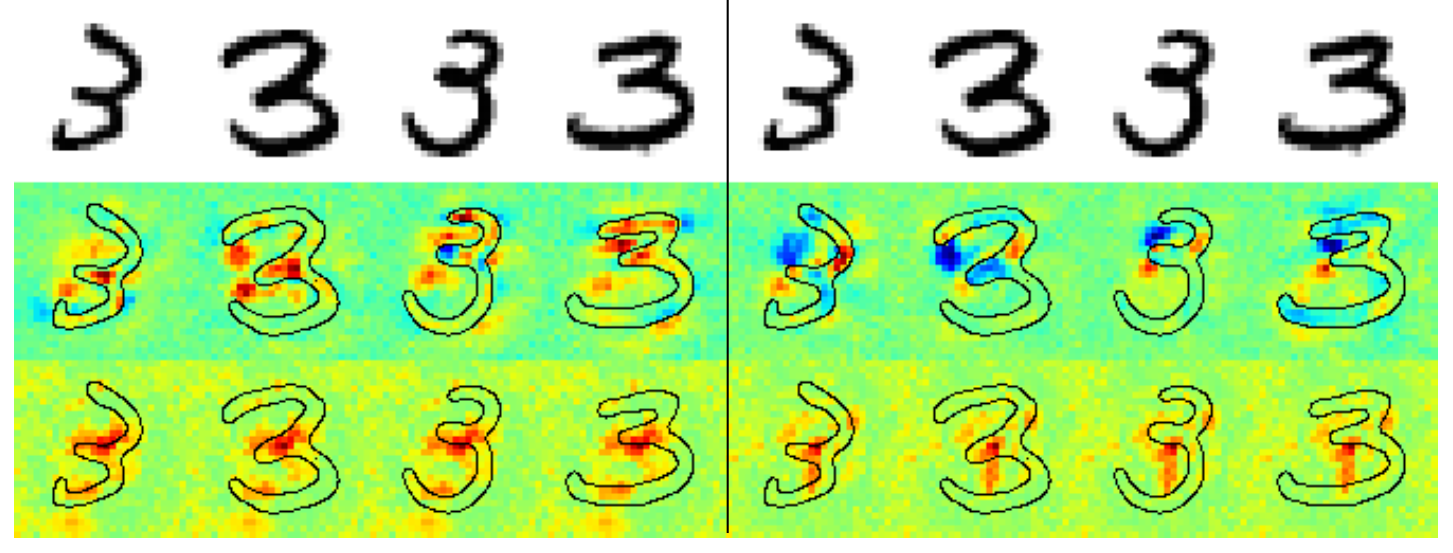
\includegraphics[width=5.8in]{header}
  \caption{3D representation of loss landscapes \protect\cite{Li2017}}
  \vspace{0.5in}
}



%% The ``\maketitle'' command must be the first command after the
%% ``\begin{document}'' command. It prepares and prints the title block.

\maketitle


%% Abstract section.

\begin{abstract}
Recent years have seen a surge in the application of machine learning, especially deep learning. These methods enable developers and researchers to solve problems which seemed too complex for traditional methods just ten years ago. However, these advances do not come without a set of unique problems. Neural networks are highly complex structures. Their internal configuration changes constantly during training and with increasing numbers of neurons. It is hard to comprehend how each individual component influences the outcome of predictions.
In this paper, we look at several ways to manage this inherent complexity by visualizing different aspects of neural networks. Approaches range from displaying a simplified version of the graph-like structure of a network to visualizing activation maps of single neurons. There are also ways to generate terrain-like plots of error functions. This is especially useful in situations where finding local minima might not be trivial.
This state-of-the-art report gives a rough overview of the wide variety of approaches to the ever-increasing complexity inherent to neural networks.
\end{abstract}

\keywordlist

\section{Introduction}
Recent years have seen a surge in the application of machine learning, especially deep learning. This is due to the fact that deep learning has seen substantial improvements over the last decades, ranging from improved algorithms \cite{LeCun1998} over the availability of big datasets such as ImageNet \cite{Deng2009} or Sports1M \cite{Karpathy} to performance improvements of modern-day GPUs coupled with flexible, and free-to-use frameworks such as TensorFlow \cite{Abadi2016} or Caffee \cite{Jia2014}.

With AI's successful application across all kinds of different tasks from detecting objects in images \cite{He2015}, to natural language processing \cite{Cho}, comes increased complexity in network architecture and structure. Today's networks contain millions of individual neurons which are hard to interpret individually. Further, since AI is being used in critical decision-making processes and EU regulations regard explanations of machine learning-based decisions as a human right since 2016 \cite{Choo2018}, visualization can be a good tool to shed light on the "black box" a neural network is sometimes referred to. \cite{Shwartz-Ziv2017}

%% The ``\copyrightspace'' command must be the first command after the 
%% start of the first section of the body of your paper. It ensures the
%% copyright space is left at the bottom of the first column on the first
%% page of your paper.

\copyrightspace

\subsection{Motivation}
As we have seen, machine learning and especially deep learning have become increasingly popular over the past years and are now being applied in a wide variety of fields. Due to the size of the input data that is necessary for training, or due to the vast number of neurons most networks consist of, we see there is a growing demand for conveying lots of information in a comprehensible way. It is highly likely that visualization might be the key to tackle this challenge.

\subsection{Visualization as a Possible Solution}
Data, especially large collections of analytical data in various fields of science, can pose enormous challenges for the people involved in analyzing these data. Datasets often exceed the limits of intuitive comprehensibility (e.g. ImageNet \cite{Deng2009}).

One approach that is frequently used to surmount these large amounts of data is visualizations. They are a powerful tool to categorize, classify, analyze and visually process data to make it more understandable. For instance, when looking at data in tabular form, it is typically harder to grasp its meaning as opposed to looking at the same data processed as a graph or bar chart.

The problem we will be discussing in this paper is the usage of visualization techniques for processing data that comes from neural networks. These include approaches form visualizing networks as a whole, over showing a graphic representation on a neuron-level to meta-level approaches, where information about network parameters is shown on a meta-level.

\subsection{Our Contribution}
With this work, we aim at informing the reader about current problems in the field of machine learning with special focus on deep learning and on state-of-the-art visualizations that are currently being applied to aid experts, as well as untrained users. We will explore how every method works individually and give a comparative overview of approaches and concepts.

\section{Neural Network Basics}
In this section, we will provide a short introduction to the basic ideas of machine learning with a special focus on deep learning.

\subsection{Neuron}
A neuron with regards to machine learning is regarded as one basic computational unit that applies a linear transformation to its previous inputs.

\subsection{Layer}
A layer represents a cluster of multiple neurons that perform the same computation with different parameters. Layers typically take on a specific function. CNNs, for example, usually feature alternating convolutional and max-pooling layers. 

\subsection{Activation}
Activation in machine learning is occurring when the input value of a neuron reaches past its threshold. This threshold is determined by the activation function. When analyzing images, a high activation directly correlates to a certain image feature being detected by a neuron.

\subsection{Machine Learning}
Traditionally, computers were designed to be programmed with specific instructions, which had been executed in an orderly fashion.
Machine learning changes these paradigms drastically. The core principle of machine learning is that computers are shown data which they are then to interpret. Through adequate ground truth data and error functions, the computer is given feedback about its performance and can therefore adjust. After a varying amount of time, the trained computer will have adapted to the underlying structure of the data enough, so that it can make educated predictions about previously unseen input. What these procedures are programmed to do is to approximate a pre-defined goal. This concept is best portrayed by an example:

Assuming the goal is to identify handwritten numbers, the machine learning algorithm is provided with the raw image of the written symbol. At first, it will guess at random which number was represented by the drawing. 
After each guess, it receives the correct answer. It then adjusts its parameters to fit the desired outcome.
This process is repeated many times with different symbols until the parameters are adjusted so precisely that the algorithm -- which is called a "model" in the machine learning domain -- can detect any arbitrary handwritten number.

The example above is fairly simple but this process works for any task designed to identify or classify data, given enough raw input material. A more significant application, may be to classify histological images in terms of cancerous cell expression, which could lead to early diagnosis of tumors.

\subsection{Deep Neural Network (DNN)}
A deep neural network is a network of linked computational nodes, aiming to mimic the way our brain works. Each node has input and output channels and a function \textit{F} to determine output from input. Neural networks are a sub-category of machine learning that builds upon its basic concepts. Only in recent years, it has become possible to use vast DNNs due to the increased performance of modern-day GPUs. Since those networks can house millions of parameters and with deep learning being applied in nearly every area of today's problem-solving, the need for visualizations in this area is steadily increasing. Therefore, DNNs are sometimes regarded as \textit{black bloxes} with no clear insight into their decision-making process.

\subsection{Convolutional Neural Network (CNN)}
A CNN is a subcategory of a DNN. The name comes from its convolutional layers which are smaller representations of the original image matrix that have been transformed by a kernel moving over the image. The convolution step is then followed by a pooling step that further reduces image size. This, in the case of max-pooling, is achieved by only using the maximum value in a certain neighborhood, which is also responsible for noise reduction.

\section{Method}
While machine learning has been applied to lots of problems in the past, recent years have seen an unprecedented rise in the application of neural networks for problem-solving, especially with the ongoing hype of deep learning. Due to this rise, visualization approaches have lacked behind, rendering machine learning to be this oftentimes so-called \textit{black box}. Hence, publications that are older than a few years may not portray the current landscape of machine learning visualizations correctly. This is why in this state-of-the-art report, we aimed to find the most recent papers on the topic and also tried to include approaches from Google, arguably one of the most important players in today's machine learning field.

\subsection{Sources and Search Strategies}
For choosing the works we wanted to include in this state-of-the-art report, we chose IEEE Xplore, Google Scholar, and Elsevier as our primary sources. Relevant publications were mainly obtained from the websites of Springer, the Cornell University Library and IEEE Xplore.

In order to make our results reproducible, we list our search terms in a list below.

\begin{multicols}{2}
\begin{itemize}
\item machine learning
\item deep learning
\item neural network
\item deep neuronal network
\item artificial intelligence
\item layer visualization
\item neuron visualization
\item deep visualization
\item data visualization
\item graph visualization
\item interactive visualization
\item user interaction
\item flow layout
\end{itemize}
\end{multicols}

Those terms were either used on their own or in combination with others.

\subsection{Criteria and Constraints}
The search terms listed above reveal a large number of publications relevant to neural network visualization, which is why we will briefly explain how we decided on the papers that were included in our work.

Since not every paper about machine learning is also discussing visualization, we discarded those that were not specifically focussed on the visual representation of data. Further, as discussed above, we only took papers into consideration that had a fairly close publication date to 2019, which is why the \textit{oldest} publication we used for this state-of-the-art report was released in 2015. Also, we aimed at only using papers that had a high citation count which is a common measure to evaluate the importance of a publication.

To choose literature relevant for this STAR we first read through the abstract of every publication on our shortlist. Then, by also reading the conclusion we decided which publications were significant to this work.

\section{Overview of Works}
This section will give a complete overview of all the work covered in this report. Each paper will be outlined shortly and notable features will be described in more detail. We have categorized works into four big categories -- structure-, feature-, metrics- and loss and error visualizations.

\subsection{Network Structure Visualization}
Works in this category mainly focus on conveying the structure and architecture of neural networks.

\subsubsection{TensorFlow's Visualization API}
Because Google is one of the major players in today's machine learning field, this section will address how their platform TensorFlow incorporates visualizations to aid its users in better understanding the underlying metrics and parameters of their deep learning models.

In their paper, Wongsuphasawat et al. explain the design and background of the visualization process Google's API uses to give users a visual overview of their underlying neural network structure and dataflow \cite{Wongsuphasawat2018}.

Because these kinds of models can contain well over thousand of low-level components -- each with individual parameters -- standard layout techniques such as flow layouts can produce diagrams that are difficult to read. Therefore, TensorFlow is bundled with a Graph Visualizer that, according to user feedback included in their paper, enhances the comprehensibility of model structures.

\paragraphbr{Goals}

To gain a good understanding of what potential users might find helpful when visualizing their networks, Wongsuphasawat et al.~consulted people involved in machine learning. Results suggested the importance of the following points:

\begin{itemize}
  \setlength\itemsep{0em}
  \item Overview of high-level components
  \item Differentiation and similarities of components
  \item Examination of nested structures
  \item No referring back to code to gain knowledge of details
\end{itemize}

\paragraphbr{TensorFlow Graph Visualizer}

Wongsuphasawat et al.'s visualization approach are based on a standard flow layout algorithm that was introduced by Sugiyama et al., representing directed graphs in a flow layout \cite{Sugiyama1981}. This method of visualizing graphs (Figure \ref{fig:sugiyama_method}) first removes cycles as well as layers and orders nodes. Afterward, coordinates are assigned.

\begin{figure}[H]
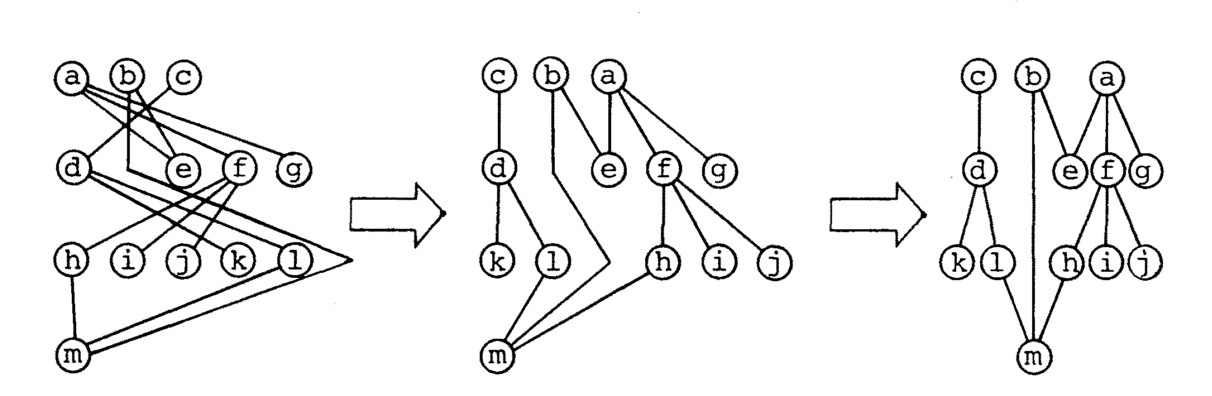
\includegraphics[width=2.75in]{sugiyama_method_sugiyama_et_al}
\caption{Sugiyama's method for visualizing graphs \protect\cite{Sugiyama1981}}
\label{fig:sugiyama_method}
\centering
\end{figure}

After this pre-processing phase, a series of graph transformations are applied to make illegible graphs easier to read (Figure \ref{fig:transformations}). \\

\begin{figure}[!htb]
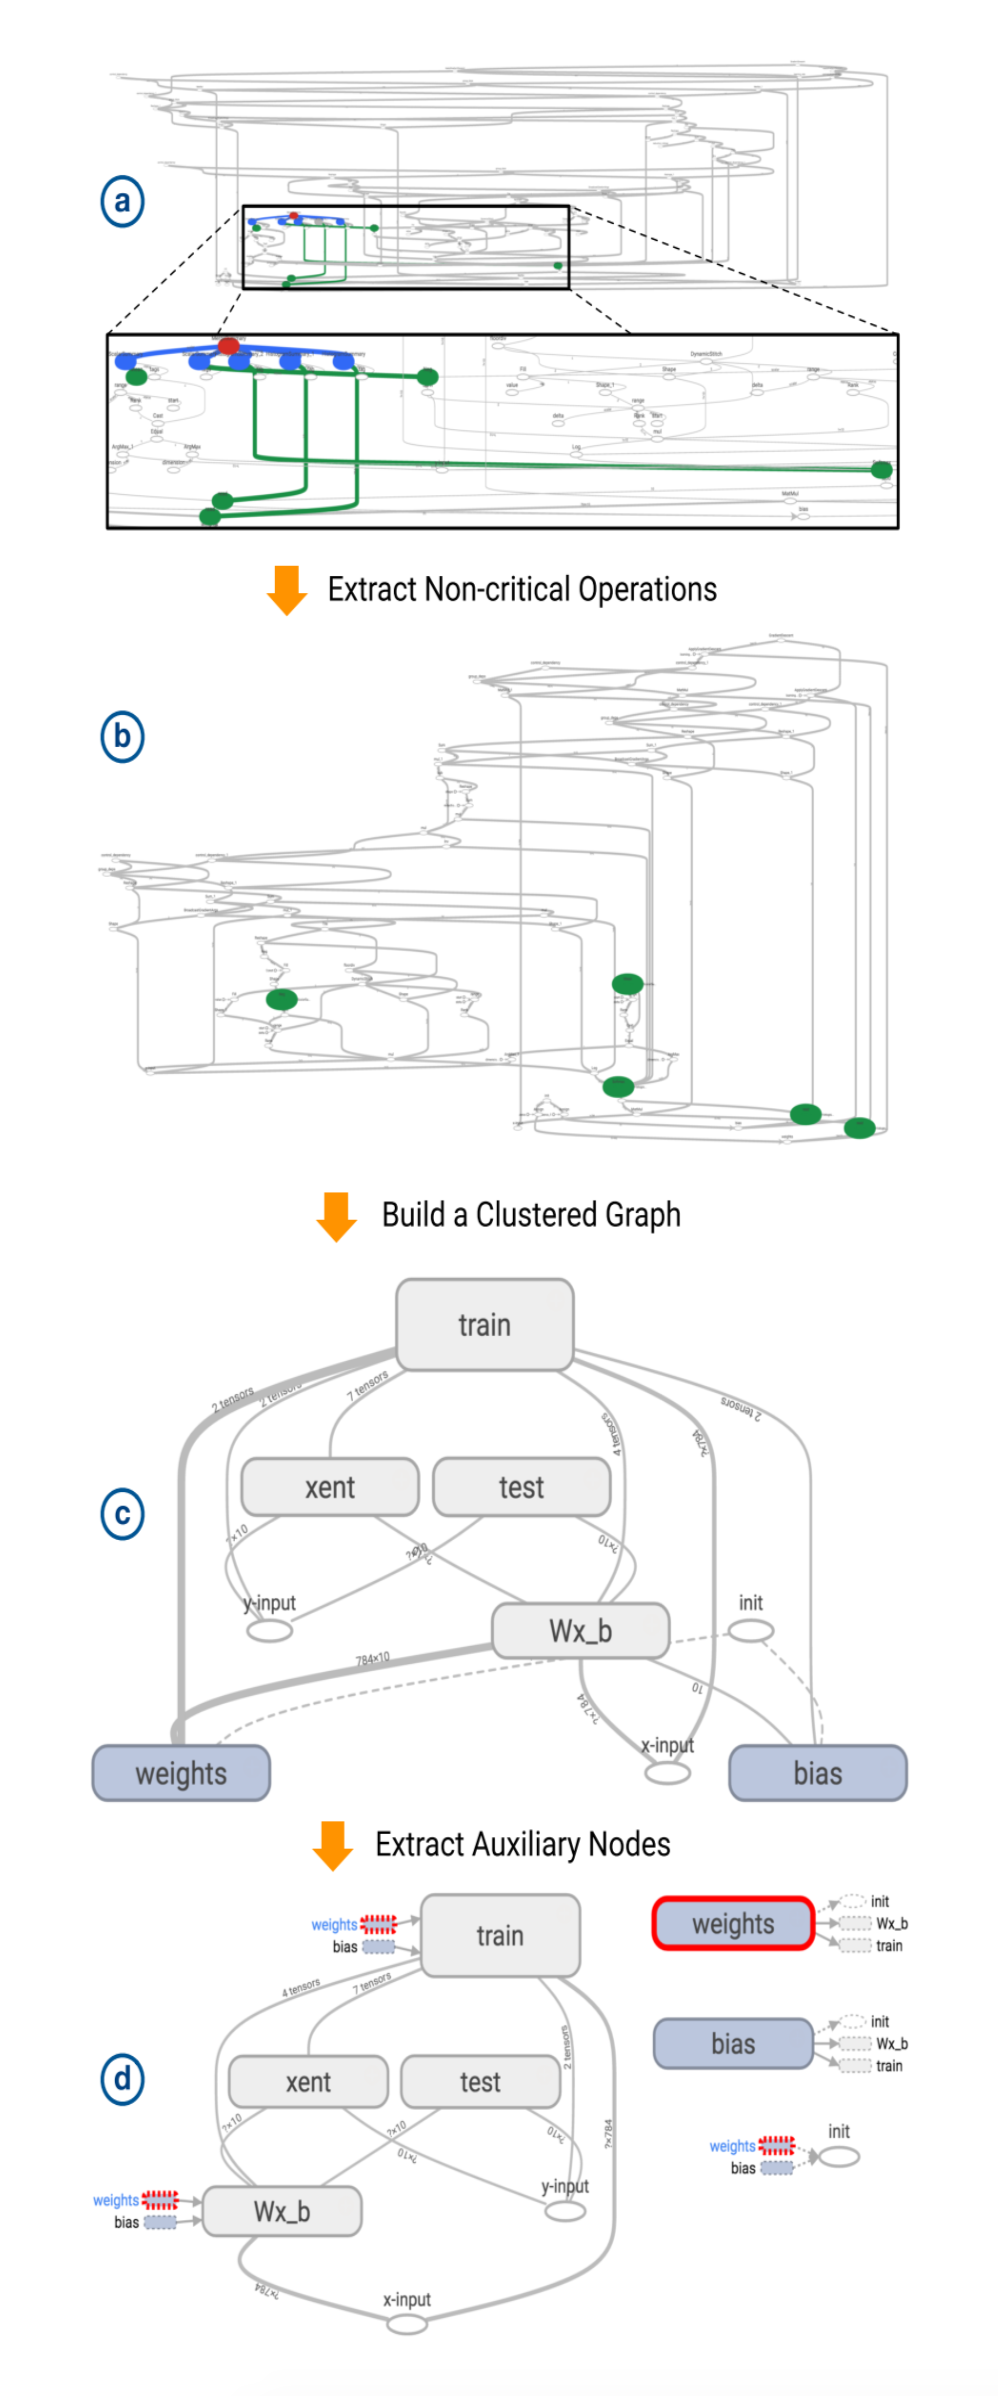
\includegraphics[width=2.75in]{transformations_Wongsuphasawat_et_al}
\caption{TensorFlow's graph transformations \protect\cite{Wongsuphasawat2018}}
\label{fig:transformations}
\end{figure}

First, non-critical operations are de-emphasized by extracting them from the layout and depicting them as either small circles or bar chart icons, depending on their role. The paper states, that those operations account for approximately 30\% of a typical network.

In the second phase, edges are bundled and a clustered graph is formed. Here, edges only connect nodes that are siblings in the hierarchy. This ensures that on interaction only subgraphs need to be refreshed, saving resources and improving responsiveness. Rounded rectangles represent group nodes, that are grouped by unique namespaces, such as "train".

As in the first step, in the third stage, non-critical nodes are extracted from each subgraph, rather than from the graph as a whole. Extracted nodes are thereby placed on the right side, as shown in Figure \ref{fig:transformations}d. Connecting nodes are also represented and give additional information when hovered over. A set of heuristics is used to determine non-critical nodes, including searching for declaring and initializing variables.

As can be seen in Figure \ref{fig:transformations}, this process declutters the graph by a high degree. Since Wongsuphasawat et al. use heuristics in some cases, unwanted results can be overruled by the user afterward.

\paragraphbr{Feedback}

Wongsuphasawat et al. gathered internal and external feedback regarding this visualization approach. Unfortunately, their paper doesn't provide any kind of statistical evaluation, thereby rendering a scientific comparison useless. According to them, internal feedback gathered by questionnaires was overwhelmingly positive, whereas anonymous feedback found online had a "positive undertone" \cite[p.~9]{Wongsuphasawat2018}.

\subsubsection{TensorFlow Playground}

In their paper, Smilkov et al. describe how Google's TensorFlow Playground aims at giving non-experts a quick and easy way into deep learning \cite{Smilkov2017}. Since the inner workings can sometimes become hard to read and interpret, the goal was to offer an interactive demo of an already trained deep neuronal network. TensorFlow Playground is an open-source in-browser tool that wants to give "novices with mathematical and practical intuition" \cite[p.~1]{Smilkov2017} a shortcut to understanding the basics of machine learning.

Their tool offers a network diagram of a DNN that is designed to solve classification or regression problems. As we can see in Figure \ref{fig:tensorflow_playground}, a circular shape with blue and orange dots can be used as training data. Two abstract features, x\textsubscript{1} and x\textsubscript{2} are then used to generate the gradient that can be seen in the neurons. In this way, users are able to see the different stages of data discrimination within the structure of a neural network. The combination of all neurons is then used to generate a heatmap on the right site that represents the output of the network. With more iterations and therefore more training, one can see, that the blue dots are separated better from the orange ones over time, giving a visual representation of the mathematics underlying the network.

\begin{figure*}
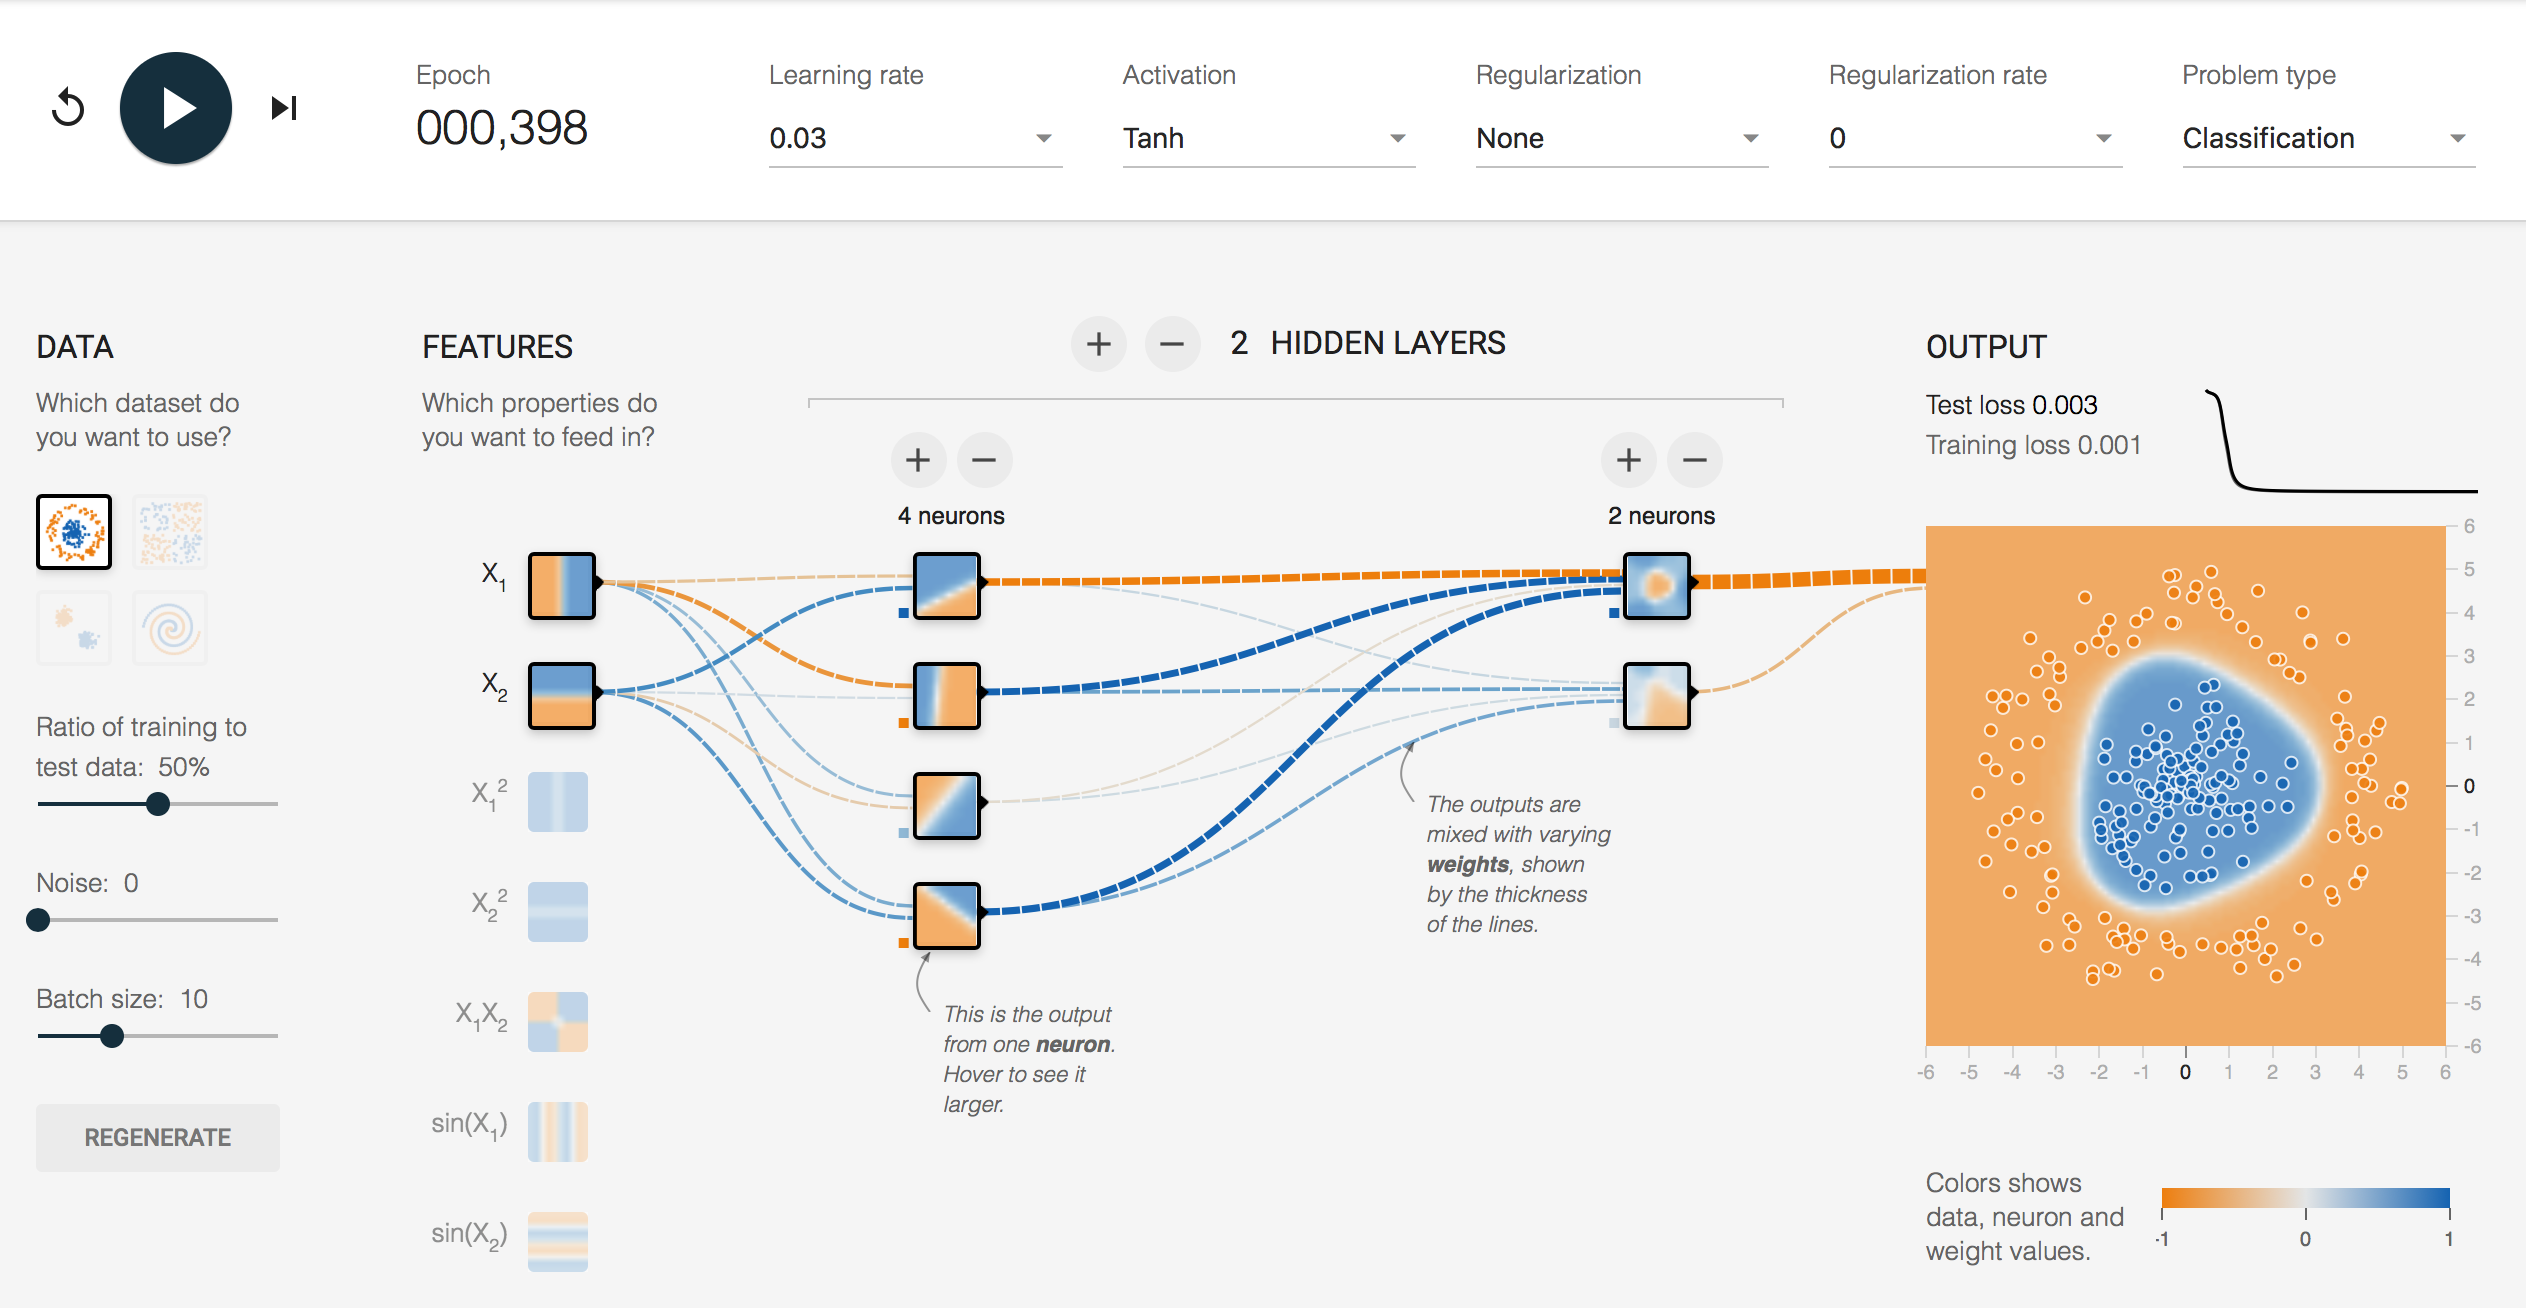
\includegraphics[width=\textwidth]{tensorflow_playground_smilkov_et_al}
\caption{TensorFlow Playground \protect\cite{Smilkov2017}}
\label{fig:tensorflow_playground}
\centering
\end{figure*}

Smilkov et al.'s playground offer people, as for example students, an easy way to experiment with a network without any prior coding experience. While the mathematics behind deep learning can sometimes feel overwhelming for newcomers, their website offers a much more straight-forward approach to the visualization of complex functions. According to their paper, TensorFlow Playground has gained positive reactions on the internet, although no statistical evidence was offered to support their claim.

\subsection{Network Feature Visualization}
Works in this category focus mainly on visualizing detected features and relevancy mappings.

\subsubsection{Multi-Neuron Activations}
Another way to interpret visualization of DNNs is to give a visual representation of the layers a network uses for its decision making.\\ 
In their paper, Yosinski et al. describe tools they developed, that enable the user to see what each neuron "sees", or expects to see, thereby making it easier to understand what a network actually interprets on the level of single neurons \cite{Yosinski2015}.

\pagebreak
\paragraphbr{Concept}

Yosinski et al.'s method use the input of a webcam to demonstrate the activation function, which is the optimal activation for each neuron respectively. This can be thought of as the input (image) that a neuron expects to see. These visual cues are then used to generate the final decision a network makes about a certain input.

\begin{figure}[H]
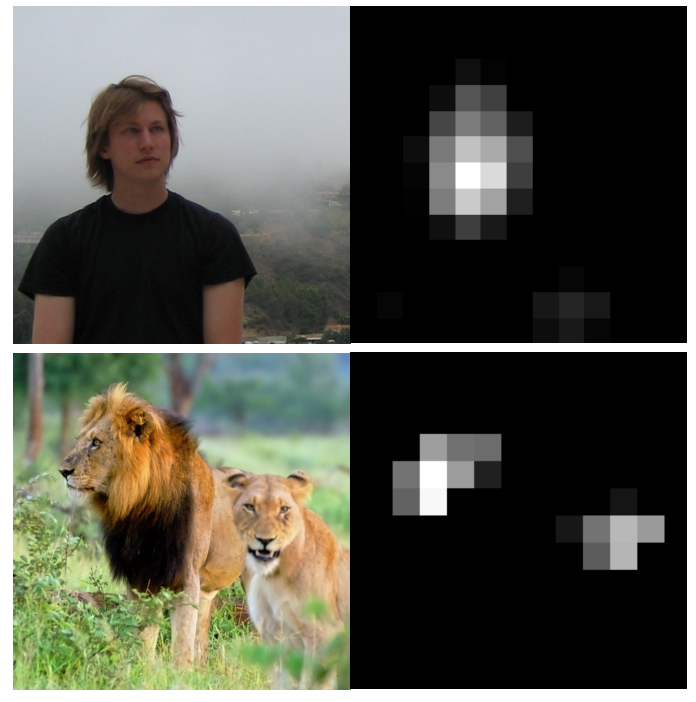
\includegraphics[width=2.75in]{detection_yosinski_et_al}
\caption{Activations for faces in a DNN trained to recognize human and animal faces \protect\cite{Yosinski2015}}
\label{fig:face_detection}
\centering
\end{figure}

As an example, a network that is trained to classify human and animal faces can be used to gather knowledge about the role each neuron plays in a network. In Figure \ref{fig:face_detection}, parts of the relevant input images can be seen. The images on the right side show which parts of the input images (left) matter for the classification of this DNN. The conclusion the authors drew from this analysis is that layers appear to be quite local, meaning that instead of the expected distribution on all layers, there are specific neurons that show a higher reaction to, for example, edges. Thereby, they create detectors for more complex concepts together with other neurons. Different local feature detectors can then make up whole objects, such as animals. \\
Visualizing these attributes of machine learning models can yield unexpected results. For example, a network that was trained to detect environments, such as playgrounds, shows some layers that are primarily activated by faces of children, even if this particular feature was not trained intentionally.\\\\
The second matter of interest in their work was the introduction of regularization options that help to generate images that are visually better interpretable.\\
Firstly, a decay function is used to decrease the importance of high values that otherwise would change the bias into an unfavorable direction. Secondly, a Gaussian blur is applied to filter high frequencies out of the input. If included, those high frequencies would result in generally favorable high activations but would at the same time decrease interpretability of the neurons attributes. Next, pixels that contain information close to zero are thresholded, since they usually do not contain relevant features. Further, the authors clipped pixels that only led to low activation to zero.\\
Yosinski et al. offer their project as open-source interactive tools, thereby making DNNs more accessible for everybody interested in seeing what a DNN actually "sees".

\subsubsection{Regional Relevance Visualization}
Similar to the paper discussed above, Samek et al. are also proposing an approach to visualize regional perturbation leading to a recognition decision via heatmaps \cite{Samek2017}. \\
To demonstrate what specific regions or features of an image are of greater or smaller importance, they compare three ways of generating heatmaps:

\begin{itemize}
  \setlength\itemsep{0em}
  \item Sensitivity Analysis
  \item Deconvolution Method
  \item LRP Algorithm
\end{itemize}

Sensitivity heatmaps utilize sensitivity analysis. This means that the local sensitivity is used to demonstrate what, for example, makes a bird more or less likely to be interpreted as a bird. Therefore this method shows how small changes in a single-pixel value influence the output of a network as a whole. Large values indicate that a pixel has a severe effect on the classification function. Since this approach focuses on local features, global features are underrepresented, leading to the drawback that the generated heatmap does not fully explain the classification of an image.\\\\
Deconvolution heatmaps are based on the concept of mapping activations of a network's output to pixel space via backpropagation. This method will, at first glance, give reasonable explanations of a decision, since the heatmap shows a matching input pattern for a classification object, meaning that the contours of a bird will be highlighted. The downside is, that, according to Samek et al., there is no direct correspondence between the generated scores and the contribution of an individual pixel to the overall decision.\\\\
Relevance heatmaps appear to be the most promising approach. They use Layer-wise Relevance Propagation (LRP) to deconstruct a decision into the relevances on a pixel level, therefore showing the contribution of an individual pixel to the end-result. This technique, compared to sensitivity heatmaps, is far more favorable towards global features and shows both, local and global impact in its heatmap. The most apparent benefit of LRP heatmaps is, that they not only visualize the positive evidence for a certain classification but also show what pixel data had a negative impact on the decision. In the example shown below (Figure \ref{fig:heatmap_numbers}) we can see that LRP, compared to deconvolution, highlights positive evidence as red, but also negative evidence, that, for example, speaks against the decision that the given image represents a "9".

\begin{figure*}
\center
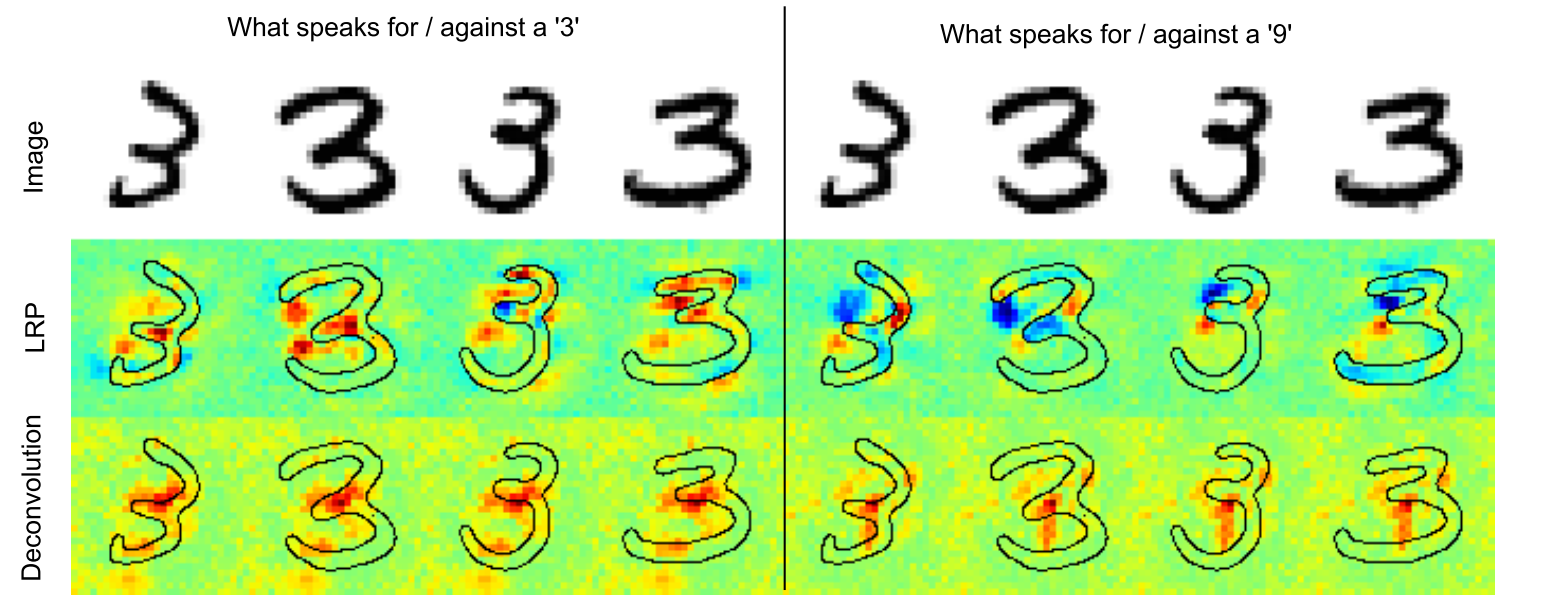
\includegraphics[width=\textwidth]{heatmap_samek_et_al}
\caption{Heatmaps for classification of numbers where red means that these areas strongly speak for the requested pattern whereas blue denotes areas that speak against that pattern \protect\cite{Samek2017}}
\label{fig:heatmap_numbers}
\end{figure*}

\subsubsection{Multifaceted Feature Visualization}
In neural networks, each neuron detects one or more features that are further propagated for the decision-making process. 
Individual features can be visualized as can be seen in the previously discussed publications, but so far we have not covered the visualization of multifaceted features in a single neuron. 
In their paper, Nguyen et al. discuss the importance of visualizing those for more complex scenes, where multiple features achieve the highest activation in a neuron \cite{Nguyen2016}. 
Previous work \cite{Erhan2009}, they state, did not take those multiple facets into consideration, which led to mixes of e.g. colors or objects. 
Therefore, their work focusses on demonstrating an algorithm that produces synthetic images that correspond with the highest activation of a neuron (Figure \ref{fig:multi}). 
For example, a bell pepper classifier has to deal with red, green and yellow bell peppers. 
So there may be different images (facets) that achieve optimal activation. 
In this case, differently colored and oriented bell peppers. 
So there is no one single image that creates maximum activation. 
The aim of this work was to create representations that take this attribute of classifiers into account and give a more accurate depiction of optimal, multi-faceted inputs.

\begin{figure}[H]
\center
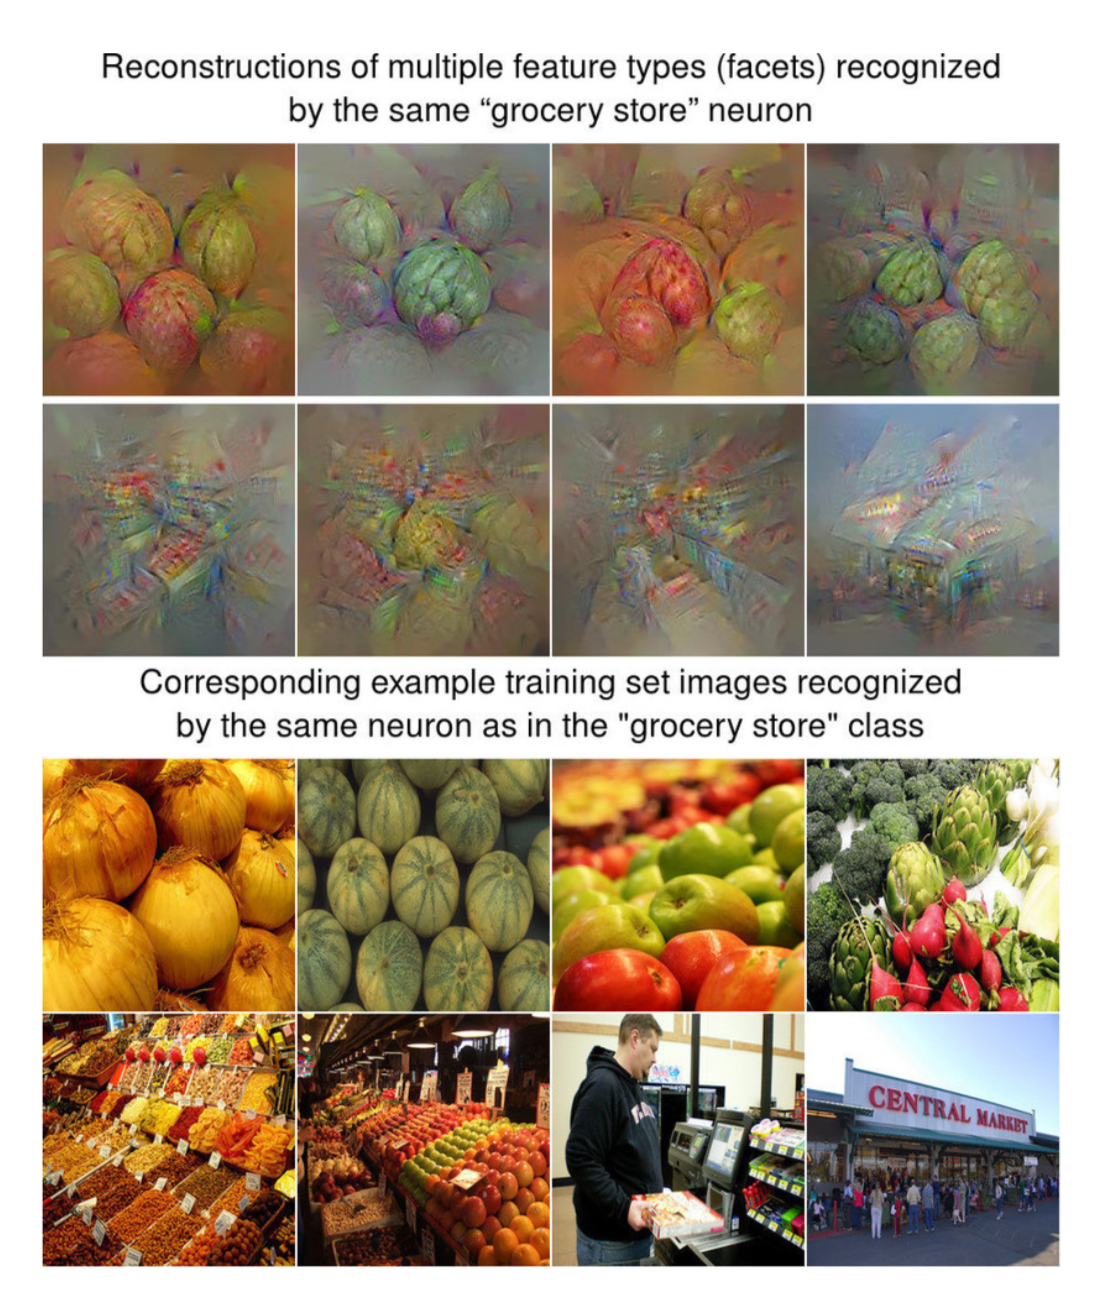
\includegraphics[width=2.75in]{multi-facet}
\caption{On the top, there are eight feature facets that activate the same neuron which was trained to identfy grocery stores. Those images were synthetically created. On the bottom, the corresponding training images that were used for initial training \protect\cite{Nguyen2016}}
\label{fig:multi}
\end{figure}

\pagebreak
\paragraphbr{Concept}

Nguyen et al.'s deep visualization approach relies on a CaffeNet-based architecture DNN that was trained on the ImageNet dataset. They use an optimization algorithm that aims at optimizing the color-values of the pixels in an image to achieve maximum activation in a given neuron.

Simplifying the approach for the sake of this state-of-the-art report, their algorithm uses a DNN's abstract knowledge of a class. This information is then clustered, which yields several clustering centers, which all represent different facets of this particular classifier. To obtain the maximum activation image of a facet, the centroid of the cluster is calculated and conventional input maximization techniques are used to produce a part of the final representation. This process is repeated for all cluster centroids to obtain the final, combined representation of the multi-faceted maximum input.

\begin{figure}
\center
\includegraphics[width=2.75in]{facet_cluster}
\caption{Illustration of the facet cluster from which the final facetted representation is generated \protect\cite{Nguyen2016}}
\label{fig:facet_cluster}
\end{figure}

An example of such a facet cluster can be seen in Figure \ref{fig:facet_cluster}.


\subsection{Network Metrics Visualization}
Works in this category focus mainly on visualizing neural network metrics such as loss or activations in a layer.
%% TODO: New content goes here Liu2016, Liu2018, Wang
\subsubsection{Towards Better Analysis of Deep Convolutional Neural Networks}
In their paper, Liu et al. introduce a  visualization approach for visualizing deep convolutional neural networks (CNNs) \cite{Liu2016}. CNNs present a major challenge for scientists and experts working with them for a number of reasons as detailed in their work. First, neural networks can consist of hundreds of individual layers that themselves are made up of thousands of neurons. This inherent problem makes analysis on a neuron-level difficult. Secondly, training CNN is a time-intensive task, where training can last for hours, days, or even weeks. Therefore, the correct identification of potential problems is key to saving time and resources.\\

\begin{figure}
  \centering
  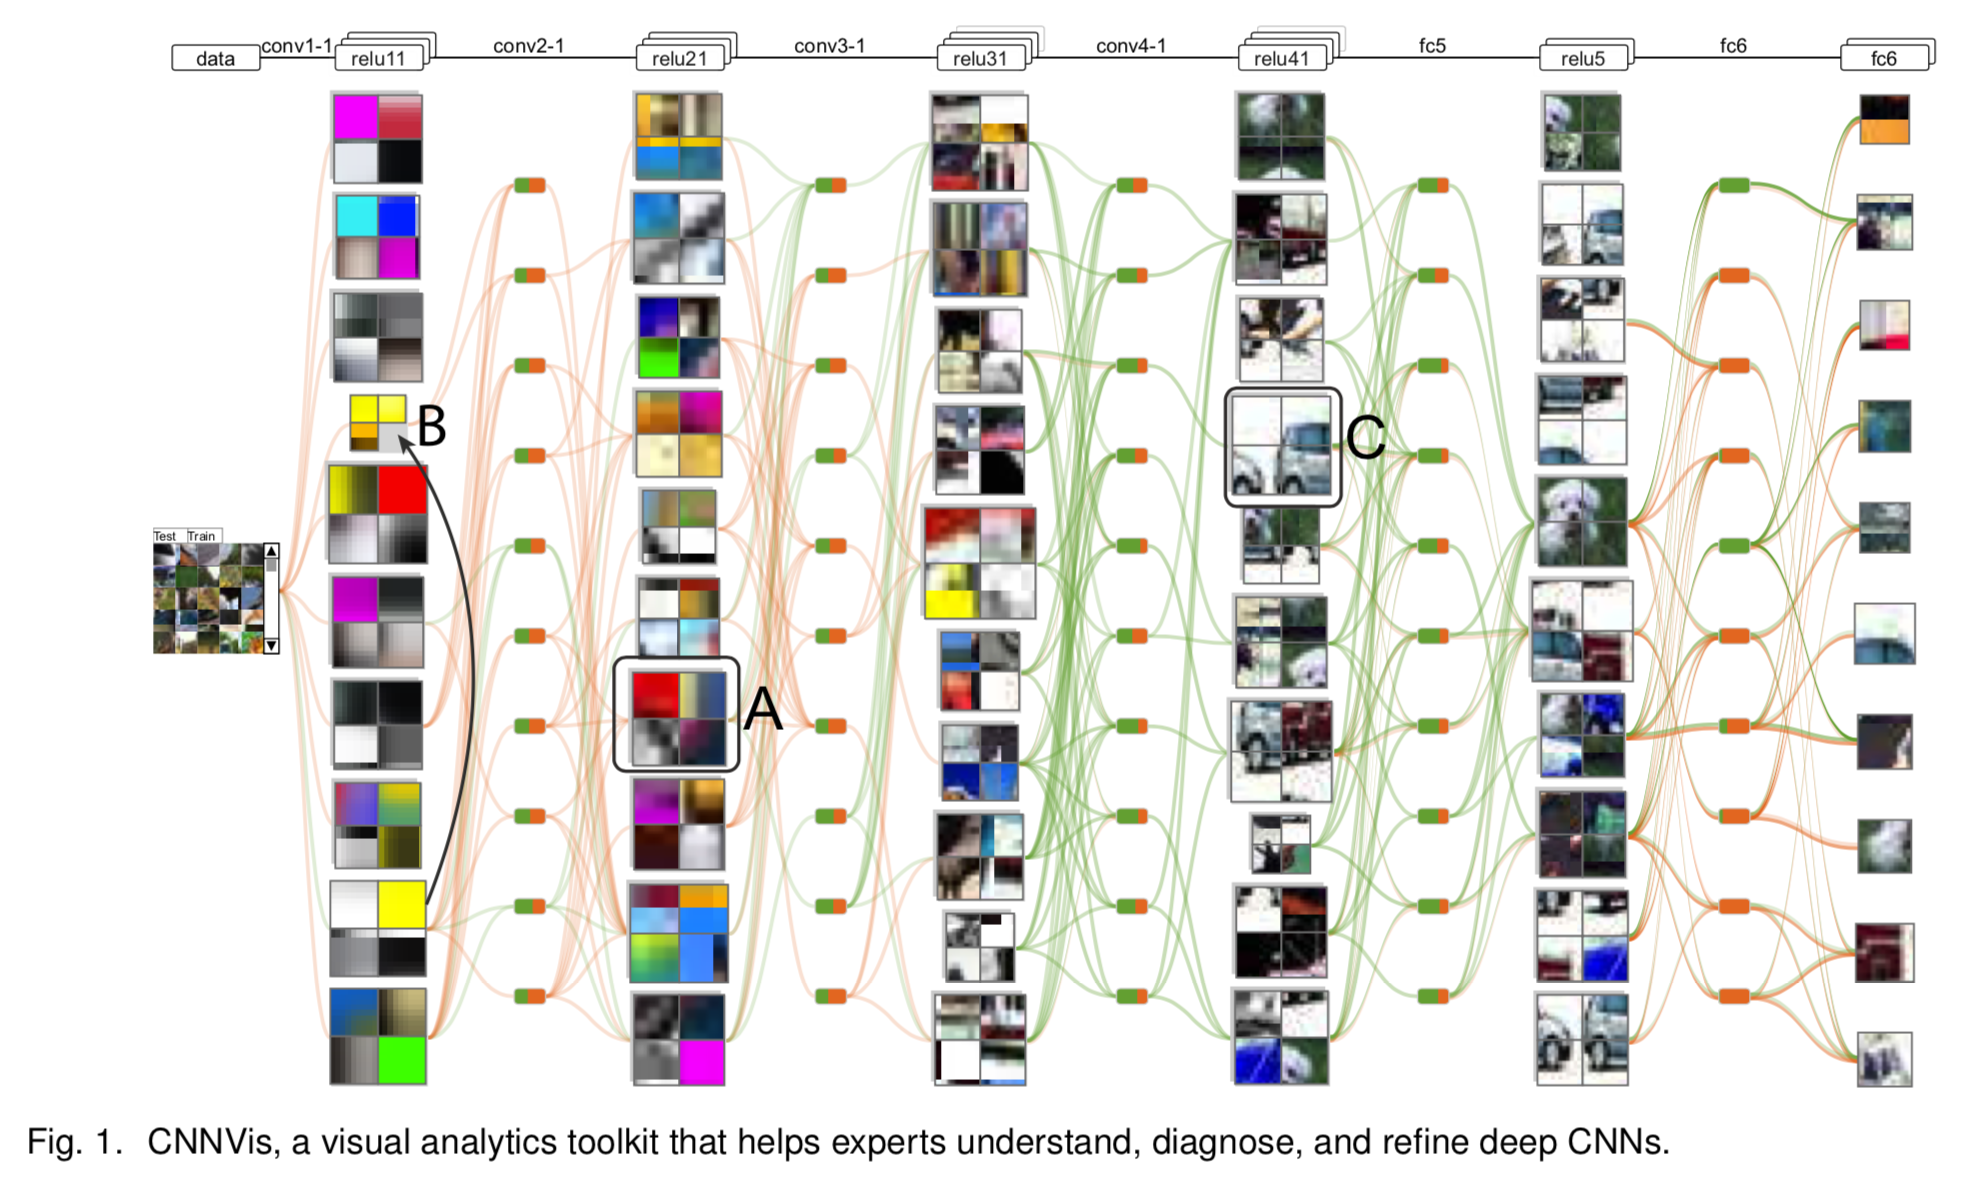
\includegraphics[width=2.75in]{cnnvis}
  \caption{Sample image of CNNVis. \protect\cite{Liu2016}}
  \label{fig:cnnvis}
\end{figure}

With their approach, CNNVis (\ref{fig:cnnvis}), Liu et al. try to tackle those challenges in order to give experts a tool for easy visual analysis of their networks. Their text describes how CNNVis works and evaluates it in three user-studies where they measure performance improvements across multiple neural networks.\\

\paragraphbr{Approach}

CNNVis uses a number of different steps to achieve a comprehensible CNN visualization. Those include the following.

\begin{itemize}
  \item The network is converted into a directed acyclic graph (DAG)
  \item Layers are clustered
  \item Representative layers are chosen
  \item Neurons of those layers are clustered
  \item Representative neurons are chosen
  \item A hierarchical rectangle packing algorithm is applied
  \item A matrix reordering algorithm helps with visualizing activations
  \item A biclustering-based edge bundling method is applied
\end{itemize}

Since we don't want to focus on every detail of how their process works, we'll outlay some of the steps listed above.\\

\begin{figure}
  \centering
  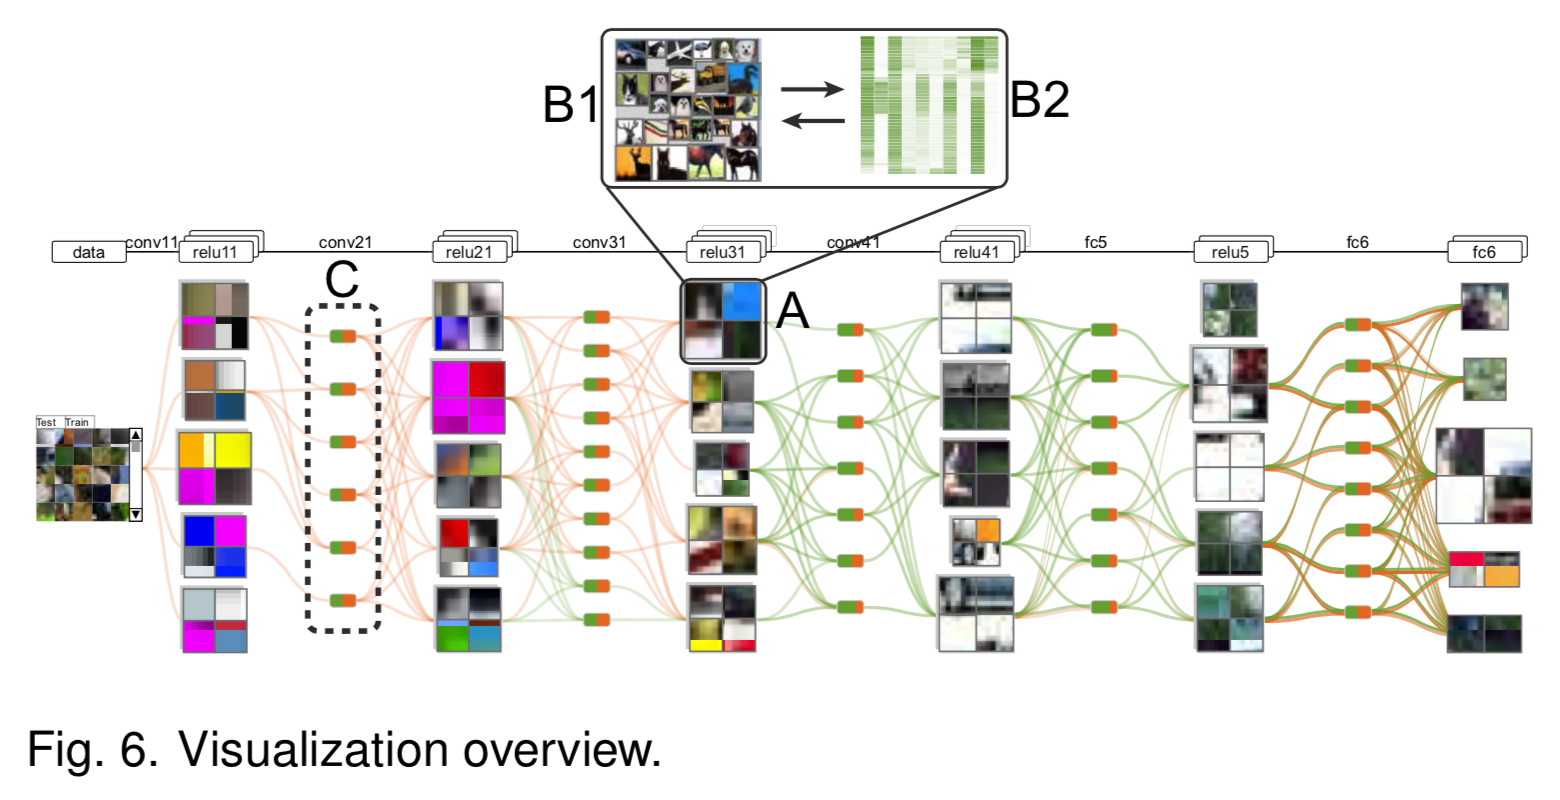
\includegraphics[width=2.75in]{cnnvis_detail}
  \caption{Sample image of CNNVis. \protect\cite{Liu2016}}
  \label{fig:cnnvis_detail}
\end{figure}

In figure \ref{fig:cnnvis_detail} we can see a detailed look at the visual output their program produces. As the input data is passed through the network, more and more features are being learned in accordance with their previous layers. Left of Figure \ref{fig:cnnvis_detail}C we can see a representative network layer with some representative neurons. The neurons are chosen by sorting for maximum activation. A pool of five neuron-clusters is picked which can be switched by the user. When clicking on an individual neuron-cluster (Figure \ref{fig:cnnvis_detail}A), the user can see how certain input images (which themselves are user-swappable) effect the activation of a single cluster (Figure \ref{fig:cnnvis_detail}B1 and B2). Through that, the features a network has learned can be understood and decisions for retraining can be made. Finally, the biclustering-based edge bundling algorithm allows for decluttering the vast number of inter-neuron connections.\\

To summarize, Liu et al.'s application is a good way to visualize deep neural networks. Their clustering techniques allow for a stripped-down exploration of a network, where only necessary components can be viewed. User interaction allows for a flexible alteration to specific user needs. To demonstrate that their approach improves many aspects of CNN training, they conducted multiple user studies. Those studies were generally favorable of CNNVis and found it to be helpful for detailed network analysis.

\subsubsection{Analyzing the Training Processes of Deep Generative Models}
In their paper, Liu et al. developed the tool DGMTracker, which allows experts to analyze deep generative models -- the most popular version being the generative adversarial network (GAN) -- at different granularities \cite{Liu2018}. 
DGMTracker offers the following three modules. Snapshot-, layer- and neuron-level analysis.
To achieve this, DGMTracker is divided into two modules. Data flow visualization and Training dynamics analysis.
Data flow visualization focuses on the general flow of input data towards the output layer. Experts can analyze hotspots and bottlenecks using this flow data. DGMTracker offers snapshot- and neuron-level analysis of data flow data.
Training dynamics are a collection of multiple parameters of interest to the expert. These include loss and average weight per layer. Those data are visualized in the Training dynamics analysis module of DGMTracker.
Using these modules the expert can then perform analysis on different levels of detail in different modalities.
An overview of DGMTracker's architecture can be seen in Figure \ref{fig:mengchen1}.

\begin{figure}[!htb]
  \centering
  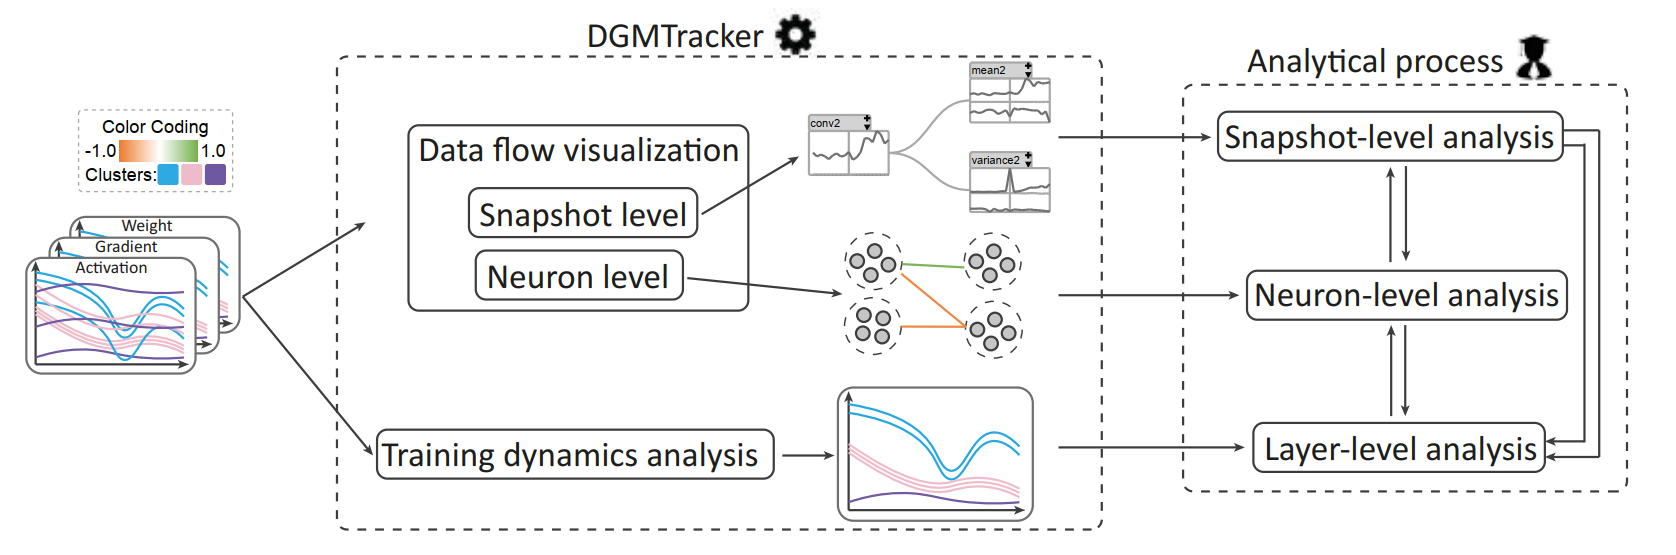
\includegraphics[width=2.75in]{mengchen1}
  \caption{Overview of DGMTracker's architecture \protect\cite{Liu2018}}
  \label{fig:mengchen1}
\end{figure}

\paragraphbr{Snapshot-Level Analysis}

Network states can be captured at different points in time during training resulting in a time series of snapshot data.
This data is usually visualized either by using dimensionality reduction methods such as t-SNE or by employing multiple line charts. 
Liu et al. relied on the latter approach, showing temporal changes in parameters such as loss or average weight in a layer (see Figure \ref{fig:mengchen2})

\begin{figure}[!htb]
  \centering
  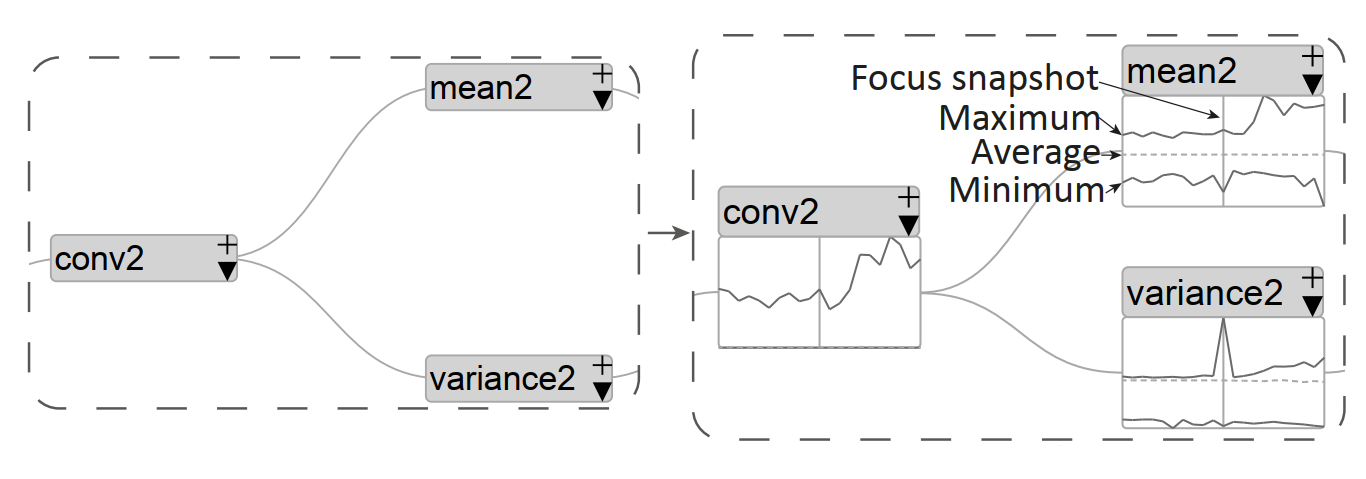
\includegraphics[width=2.75in]{mengchen2}
  \caption{Snapshot-level analysis -- each layer is portrayed as a separate area and metrics are shown within its boundaries \protect\cite{Liu2018}}
  \label{fig:mengchen2}
\end{figure}

These data cumulatively represent the overall training dynamics of a network.

\paragraphbr{Neuron-level Analysis}

On this level, the expert can see how each neuron of one layer contributes to the input of the following layer. The contribution is assessed by using a credit assignment formula which maps each node's influence to a scale of minus one to one (where negative values mean backward contribution and positive ones denote forward contribution).
These values are mapped to visual representations of the nodes through a color map. Connections between nodes follow the same scheme. Their thickness additionally shows the magnitude of contribution to individual connections. Since there are usually too many nodes in each layer to visualize them all separately, Liu et al. have used K-Means clustering to reduce visual clutter. Neurons are then placed on a feature map to further reduce complexity (see Figure \ref{fig:mengchen3}).

\begin{figure}[!htb]
  \centering
  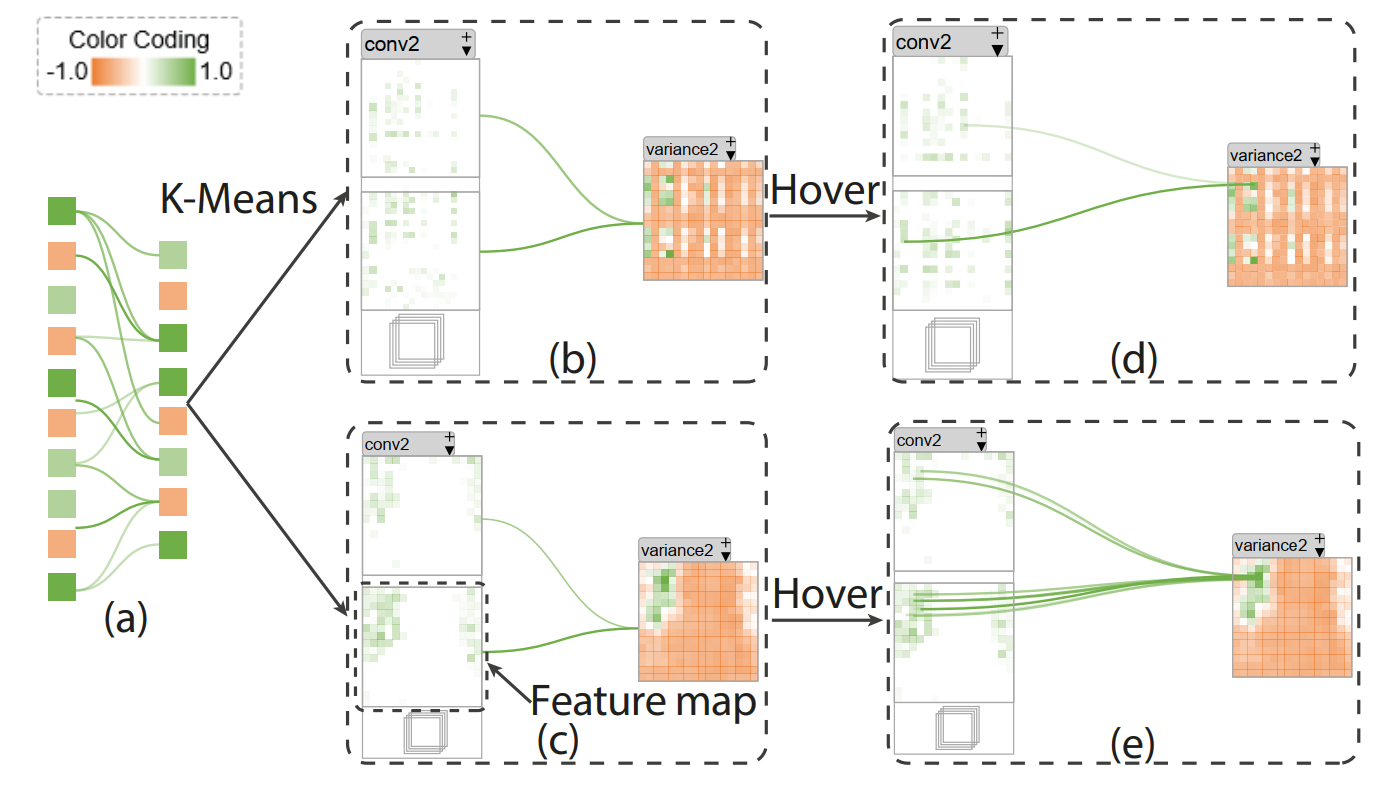
\includegraphics[width=2.75in]{mengchen3}
  \caption{Neuron-level analysis -- single node contributions are clustered using K-Means and are then mapped to feature maps to enhance legibility \protect\cite{Liu2018}}
  \label{fig:mengchen3}
\end{figure}

\paragraphbr{Training Dynamics Visualization}

This second module of DGMTracker was designed to enable experts to analyze training processes on a temporal level.
Snapshot data is visualized using different line charts showing metrics such as loss and layer activation over time. Again, visualizing all the data directly will usually lead to visual clutter. In this case, Liu et al. propose blue-noise sampling to extract a representative overview of the raw data (see Figure \ref{fig:mengchen4}). The advantage of blue-noise sampling over the conventional random sampling of snapshot data is that the former preserves outliers. This is especially important if the expert is to find layers and neurons that may cause training failure.

\begin{figure}[!htb]
  \centering
  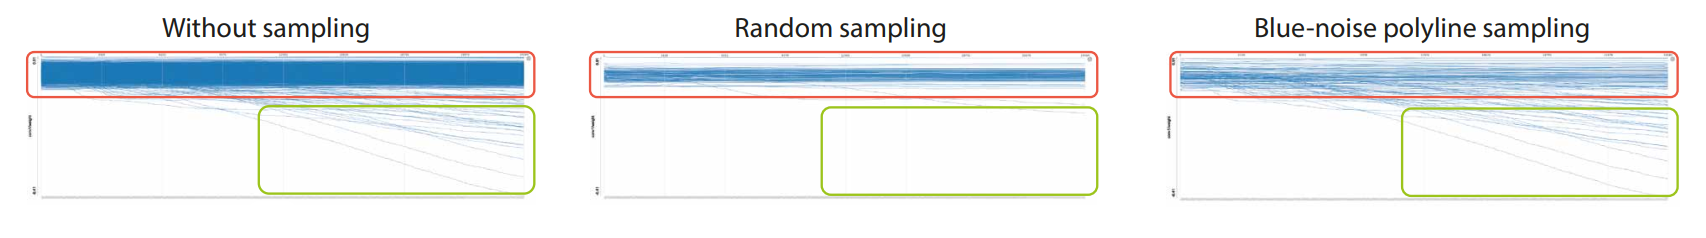
\includegraphics[width=2.75in]{mengchen4}
  \caption{Training Dynamics -- relevant data is picked from the raw data (left) using blue-noise sampling to preserve outliers (right) as compared to random sampling (middle) \protect\cite{Liu2018}}
  \label{fig:mengchen4}
\end{figure}

\subsubsection{GANViz: A Visual Analytical Approach to Understand the Adversarial Game}
Wang et al.'s paper describes a novel approach to visualize Generative Adversarial Networks (GANs) \protect\cite{Wang}. GANs, in contrast to the more commonly used CNNs, is used for image data generation, rather than discrimination. As such, they are used for generating images for DNN training in areas where the datasets used are not sufficient. Further, last year NVIDIA presented a GAN that is able to generate realistic fake portrait photos that are difficult to discriminate against real ones \protect\cite{KarrasNVIDIA}. 
GANs differ from the usual CNN architecture, as they are trained by two adversarial networks. One of those networks called the Generator (G) generates fake data that is being handed to the Discriminator (D), who tries to identify the fake. During the training-process, G is constantly developing its ability to produce sufficiently good images so as to fool D, whereas D is getting better at discerning images handed by G from the real ones mixed in the dataset.\\

In order to improve working with GANs, Wang et al. have consulted with experts on what their solution, GANViz is required to incorporate. To aid those experts, the main focus areas of GANViz are as follows.

\begin{itemize}
  \item The support for model evaluation while training
  \item Visualization of model interpretation
  \item Comparative visualization with a focus on the difference between false-positive and true-positive images (e.g. images of apples vs. oranges)
  \item Comparative visualization with a focus on tracking training data during the training process
\end{itemize}

\paragraphbr{Approach}

To achieve the goals described, we will give an overview of how GANViz works. GANViz is used to visualize deep convolutional GANs (DCGANs), which feature, as an extension of GANs, a deep deconvolutional network as G, and a deep convolutional binary classifier as D. For visualization, a multitude of parameters are being measured during training. The most important parameters for examining the training progress are as follows.

\begin{itemize}
  \item The loss function of G and D, which indicates the quality of a model as it measures the prediction error of a model;
  \item The probability values of D's discrimination with regards to the prediction of real vs. fake images;
  \item The activations from all layers for each image when being passed through D;
  \item The area under the curve (AUC) which plots the true-positive rate against the false-positive rate;
\end{itemize}

\begin{figure*}
  \centering
  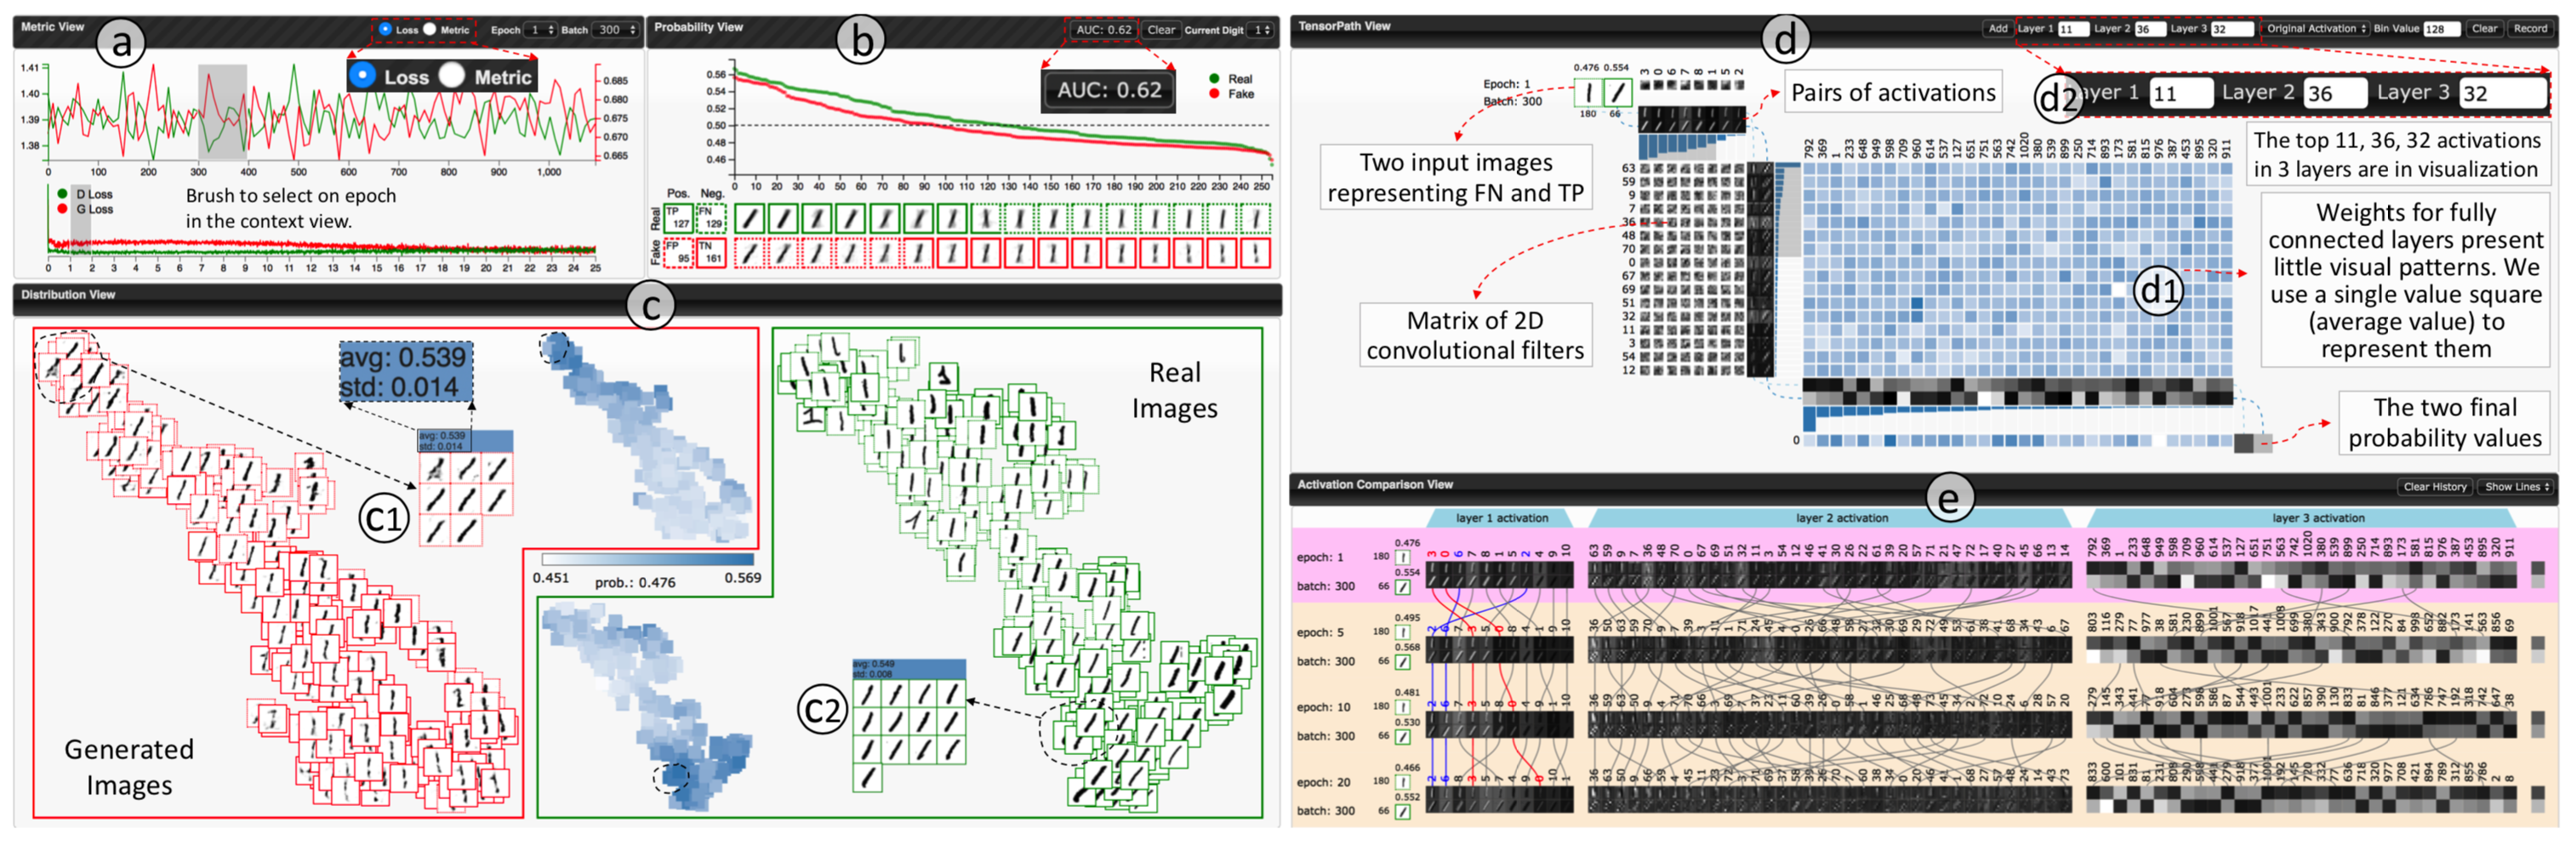
\includegraphics[width=\textwidth]{ganviz}
  \caption{GANViz -- main interface \protect\cite{Wang}}
  \label{fig:ganviz}
\end{figure*}

As seen in Figure \ref{fig:ganviz}a and b, most of those parameters are plotted as charts. The distribution-view in Figure \ref{fig:ganviz}c is used for representing the performance of G, by showing the feature probability distribution of real vs.~fake images. Here, after applying dimensionality reduction, generated and real images are plotted in a 2D graph, indicating what images tricked D by encoding the prediction probability with a color gradient. A lasso tool is implemented to give users the ability to examine specific images in detail. The TensorPath view seen in Figure \ref{fig:ganviz}d provides an overview of D's network architecture, where the activation of certain layers can be viewed individually. Further, as seen in Figure \ref{fig:ganviz}e, those activations can be compared between layers and over multiple timestamps. This activation comparison view is linked with the TensorPath view, allowing for the user to actively compare the activations of multiple images.

GANViz was evaluated in a case study and by assessing experts' feedback.

\subsection{Network Error and Loss Visualization}
In some cases, it is more desirable to explore neural networks in terms of training data and loss rather than looking at an already trained model.
The inherent difficulty when choosing a particular network architecture is knowing how hard it will be with given training data to reach a global minimum in the error function and therefore reach optimal network performance.

\subsubsection{Loss Landscapes}
Efforts have been made to visualize these so-called loss landscapes, which are essentially three-dimensional plots of loss functions \cite{Li2017}.
One problem that typically arises from these kinds of visualizations it that it is not immediately apparent to what degree changes in the network weights influence the change in error. In other words, it is hard to estimate how rough or smooth the loss landscape is. This problem is due to the scale invariance of network weights since most networks use normalization techniques. In that way, relative changes in weights and activation intensity do not play a role in the actual performance of the network. Li et al. have shown how to solve the problem of scale invariance \cite{Li2017}. In general, a smooth landscape is more desirable since chances of getting "stuck" in a local minimum are smaller than in reality "noisy", "spiky" environments. Sharpness or flatness of the minima themselves also plays a role and is, in most cases, directly connected to the roughness of the loss surface.

It is important to note that the morphology of loss landscapes highly depends on the chosen network architecture. Small changes can have a great impact on the outcome loss-wise. Figures \ref{fig:rough_loss} and \ref{fig:smooth_loss} show the same ResNet with (\ref{fig:smooth_loss}) and without (\ref{fig:rough_loss}) so-called skip connections, which are structural modifications of a standard network \cite{He2015}.

\begin{figure}
\centering
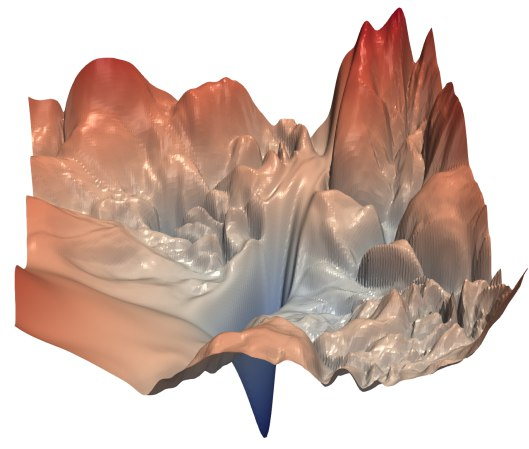
\includegraphics[width=2.75in]{rough_loss}
\caption{Rough loss landscape of a ResNet-56 \protect\cite{Li2017}}
\label{fig:rough_loss}
\end{figure}

\begin{figure}
  \centering
  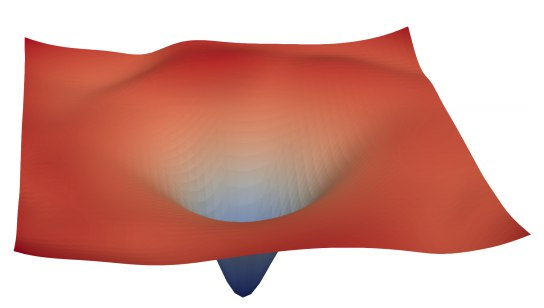
\includegraphics[width=2.75in]{smooth_loss}
  \caption{Smooth loss landscape of a ResNet-56 with skip-connections \protect\cite{Li2017,He2015}}
  \label{fig:smooth_loss}
\end{figure}

It becomes immediately clear from these examples that visualizing these landscapes can be a great benefit when developing new kinds of networks. This is because it enables researchers to see the impact of their modification at first glance. Conventionally, the use of mere mathematical descriptions of the changes may not convey this information as easily.

\subsubsection{Filter-Wise Normalization}

To address the issue of scale invariance, Li et al. proposed a method called Filter-Wise Normalization. In this approach, the loss surface is generated by evaluating the error function in random directions $d$. Conventionally, this was prone to the particular scale of the neurons. To avoid this, instead of using these directions $d$ directly, they are first normalized with respect to each individual filter/neuron.

\begin{figure}
\begin{equation}
  d \Leftarrow \frac{d}{\left\Vert d \right\Vert} \left\Vert\theta\right\Vert
\end{equation}
\caption{Simplified version of the original normalization equation, where $\theta$ denotes the network weights \protect\cite{Li2017}}
\end{figure}

This new method allows the creation of plots that are comparable among each other.

\section{Comparison}
In this chapter, we are comparing the papers presented in the previous section. 
The categories are loosely based on the work of Hohman et al. who did a comprehensive survey of the state-of-the-art of visual analytics in deep learning \cite{Hohman2018}.
In their paper, they treat the WHY, WHAT, WHEN, WHO, HOW and WHERE of visual analytics in this area.
We will focus on the WHAT, HOW and WHEN in this chapter. This means that the papers of this work will be compared and categorized based on what specific data domain of deep learning they are visualizing and what means have been used to visualize that data. Additionally, it is important to understand if this is done during or after training (WHEN).

Hohman et al. propose several categories of which we will use the following for our purpose. We omitted some and adjusted others to better fit our selection of work. A comprehensible overview of all the papers we compared can be seen in Figure \ref{fig:comparison}.

\subsection{What Data Is Visualized?}
Papers in this report can be categorized as follows based on what kind of data they visualize.
\subsubsection{Network Architecture}
Network structure visualization is one of the main parts of Googles approaches \cite{Wongsuphasawat2018,Smilkov2017}.
There are, however, other works that show the network's architecture to some degree or with higher abstraction without making it the main focus of the work \cite{Liu2016,Liu2018}.
\subsubsection{Neural Network Edge Weights}
Liu et al. in both their works \cite{Liu2016,Liu2018} focus heavily on edge weight visualization. Those were the only works in our selection that made this specific feature a major concern. As will be shown below, it is more favorable, in many cases of deep neural networks, to visualize the activation of the filter arrangement.
\subsubsection{Convolutional Filters}
These filters are mainly used in convolutional neural networks as they act on an input image like an array of small operators, extracting information about local neighborhoods in an image. TensorFlow Playground's overview -- although it is not the main feature of the project -- contains a small preview of the kind of filter that each node in the network applies to the whole image \cite{Smilkov2017}. What is missing, is a detailed and explorative tool, which lets its users examine those filters in detail.
\subsubsection{Activations}
Layer- and neuron-wise activations are one of the biggest topics in this state-of-the-art report. This is mainly due to their immediate relevance to gain better insight into a network's inner workings.
There are several approaches that focus directly on acquiring visual mappings of the activation patterns in different parts of the network \cite{Yosinski2015,Nguyen2016}. Other authors focused on showing which areas of the input affect the output of a network the most \cite{Samek2017}. Again others were concerned with showing the activations themselves without further processing those data \cite{Liu2018}. These are all different approaches to the same issue. Namely, how to input data affects the behavior of the network. One area in which such analysis is crucial is preventing adversarial attacks on networks \cite{Hohman2018}. If the weaknesses of the network are understood in detail, it can be "tricked" into producing wrong output by tweaking inputs only marginally -- many times not even noticeable to the human eye (if the input is images) \cite{Hohman2018}.
\subsubsection{Errors and Loss}
Li et al.'s work was the only paper in this report that examined the nature of errors and loss in the sense of dedicated visualizations \cite{Li2017}. One of the major advantages of this approach is that, even before training, experts can analyze the theoretical "hardness" of the training process. As could be seen, smooth loss landscapes lend themselves better to use with gradient descent optimization algorithms \cite{Li2017}.
\subsubsection{Model Metrics}
Model metrics are quite different from the previously listed categories. Metrics can be calculated from data collected during and after training and often includes loss, accuracy or aggregated activations among network layers. They tend to be less intuitive than more visual approaches but are, for some applications, more precise. TensorFlow \cite{Wongsuphasawat2018} offers its users basic metrics that are useful for everyday use while the works of Liu et al. as well as Wang et al. are highly specialized solutions intended for domain experts, since they offer a broader range of visualizations and interaction \cite{Liu2016,Liu2018,Wang}.

\subsection{How Is the Data Visualized?}
Papers in this report can be categorized as follows based on how the data is visualized -- in other words, what kind of techniques are used.
\subsubsection{Node-Link Diagrams}
Node-link diagrams can be used to represent the structure of a deep neural network. They also lend themselves to be used for data flow visualizations. This is the reason why they have become the tool of choice in many papers of this area \cite{Hohman2018}. TensorFlow visualizations use this technique to display network neurons as nodes and edge weights as edges in a graph \cite{Wongsuphasawat2018}. Bundling algorithms are used to reduce visual complexity \cite{Hohman2018,Wongsuphasawat2018}. Liu et al. also follow this trend in their solutions \cite{Liu2016,Liu2018}.
\subsubsection{Dimensionality Reduction and Scatter Plots}
Oftentimes the data that is to be visualized in machine learning lies in high-dimensional space. These high number of dimensions can simply be a part of the input data or arise from transformations within the network. Since many visualizations try to show the inner workings of a neural net, node attributes like weight are used to display some result. Since there are usually hundreds of nodes within a single layer of a deep neural net it becomes clear why authors need to employ dimensionality reduction techniques in these areas.
Nguyen et al. used the popular method t-SNE to display the different facets of a neuron \cite{Nguyen2016}. 
Aside from intra-network parameters like node weights, Li et al. use linear interpolation and contour plots with random directions to reduce loss functions in high dimensions to just 1D and 2D respectively \cite{Li2017}.
Wang et al. use t-SNE to yet another end \cite{Wang}. In their "distribution view" they give an overview of fake and real images in the generative adversarial network \cite{Wang}. To achieve this they use t-SNE for optimal image distribution \cite{Wang}. 
\subsubsection{Line Charts}
Line charts are a simple way to visualize time-oriented data. They can, therefore, be conveniently used in deep learning to display training progress via different metrics like a loss. These charts are extensively used by Google's TensorFlow visualizations as well in their TensorFlow Playground \cite{Wongsuphasawat2018,Smilkov2017}.
They serve the same cause -- namely, showing the progression of training metrics -- in Liu and Wang et al.'s works \cite{Liu2018,Wang}.
\subsubsection{Notable Interactivity}
This is one of the broader categories since there are many different ways to interact with a visualization. Therefore, they are harder to compare than most other categories in this list. Since most visualizations in our list offer basic functionality like panning, zooming, filtering or edge aggregation (in cases of graph visualization), we will only mention notable examples in this section.

One fully interactive tool is, of course, TensorFlow Playground \cite{Smilkov2017}. It lets its users add and remove network nodes at will and also allows for live modifications of training and test data. TensorFlow's graph exploration, which lets users expand every part of the network visualization up to the smallest detail, should also be mentioned here \cite{Wongsuphasawat2018}.

In Yosinski et al.'s deep visualization tool, the user can select different channels \cite{Yosinski2015}. Based on this selection, detail panels are updated accordingly with details about activations \cite{Yosinski2015}.

Liu et al. allow users to select specific neurons of interest and choose different classes to show which neurons react the most to which inputs \cite{Liu2016}. In addition to this, the active facet can also be switched to better understand the behaviors of single neurons \cite{Liu2016}.
\subsubsection{Feature Visualization}
This section covers those techniques that aim to visualize what a deep neural network "sees" in its layers, or rather, what kind of input achieves the highest activation in specific neurons. What all of these works have in common is that they generate some new image based on data of neuron activations \cite{Hohman2018}.

One common task is so-called "activation maximization", where the goal is to maximize the activation of a neuron by generating input that specifically targets this neuron \cite{Hohman2018}. A recent paper in this area, which improved upon previous work \cite{Erhan2009}, is Nguyen et al.'s Multifaceted Feature Visualization which employs state-of-the-art techniques to generate hundreds of these maximal input images \cite{Hohman2018,Nguyen2016}. 

Although not strictly about definitive features, Samek et al., in their work on deep neural network visualization, generate heatmaps showing which areas of the input speak most for or against a pre-defined class \cite{Samek2017}.

\subsection{When Is the Data Visualized?}
Papers in this report can be categorized as follows based on when the data is visualized. Visualizing the data during training can be a benefit since the expert can intervene as soon as anomalies are detected. However, visualizing data after one or multiple pieces of training have finished often yields a better general overview of the data \cite{Hohman2018}.
\subsubsection{During Training (Online)}
The most prominent example of online visualization in machine learning is perhaps TensorFlow's deep learning metrics visualization \cite{Wongsuphasawat2018} as well as the TensorFlow Playground tool, which lets users interact with a simulated training process by means of intuitive visualization \cite{Smilkov2017}.
Aside from Google's solutions, the work of Liu et al. \cite{Liu2018} provides a tool to analyze deep generative models online. In comparison to the TensorFlow toolchain, it offers more options for interactions and refined analysis. Another solution that allows analysis in more detailed was outlined by Wang et al. \cite{Wang}. Like Liu et al.'s work, Wang et al. worked specifically with generative models.

One candidate can be placed in both the online and offline category. Li et al.'s loss landscape visualizations offer an analysis of optimal learning path \cite{Li2017}. This feature can also be used to visualize the "route" taken on the loss landscape during training.

\subsubsection{After Training (Offline)}
This category is dominated by heat map-like approaches. The works of Samek et al. and Nguyen et al. both present ways of visualizing the networks inner workings by composing images algorithmically \cite{Samek2017,Nguyen2016}. 
Liu et al.'s work, on the other hand, focuses more on structural visualization \cite{Liu2016}.

Again, Li et al.'s loss landscapes also cater to offline analysis in the sense that they give an idea of the training complexity that is inherent to the network structure \cite{Li2017}.

\section{Summary and Discussion}
In the overview section of this report, it could be seen that there are four main categories of visualizations of neural networks. A neuronal network can be visualized on a meta-level by representing the structure of its nodes and high-level constructs in the form of graphs. Compared to that, the direct input, output and everything that happens in between can also be visualized to give the user a better understanding of the actual inner workings of a network. Another way is to visualize metrics data. In addition, the underlying loss function also lends itself to visualization as it provides insights about the feedback behavior of the network.\\
In this section, we will discuss and summarize these approaches.\\

\subsection{Network Structure Visualization}

We have looked at the way Google's TensorFlow utilizes algorithms on directed graphs to make complex neuronal networks easier to read \cite{Wongsuphasawat2018}. Because being available within their API, this is a feature that is likely to be beneficial for everyone who uses TensorFlow as their machine learning platform. As seen in Figure \ref{fig:transformations}, Google's approach makes convoluted graphs very much readable, which allows for improved analysis of neural networks. Since there is no obvious downside to their approach, it can only be noted that it would be beneficial if they would provide detailed comparisons with other emerging techniques in this area.

As seen in the work of Smilkov et al., there is a great need for visualizing the so-called \textit{black box} that neural networks can sometimes seem to be \cite{Smilkov2017}. Therefore, we discussed their method of visualizing networks for teaching and learning, TensorFlow Playground.

\subsection{Network Feature Visualization}

Yosinski et al. offer an open-source project that aims to show the visual input and interpretation from every layer to every neuron of a DNN \cite{Yosinski2015}. They, therefore, offer a very interesting insight into how a neuronal network actually generates an output and therefore classifies an image.

With their work on heatmaps, Samek et al. have shown, as Yosinski et al., that the knowledge about the workings of individual components can be quite insightful for engineers of a DNN. They proposed different ways of representing the decision-making-process of a neural network as heatmaps \cite{Samek2017}. We have seen, that there were clear advantages with some approaches, such as LRP, where even negative evidence against a decision can be shown. It seems clear that the usage of discussed techniques would be greatly beneficiary for people working on optimizing the performance of specific neural networks.

Nguyen et al. build upon previous work by Erhan et al. to offer deeper insight into the behavior of single neurons \cite{Nguyen2016,Erhan2009}. In their paper on Multifaceted Feature Visualization, they show methods to construct artificial images based on neuron activation data \cite{Nguyen2016}. These images aim to maximize the activation of certain neurons.

\subsection{Network Metrics Visualization}
%% Liu2016 Towards Better DNN Visualization
Liu et al. propose a method to visualize deep convolutional neural networks using a simple graph layout \cite{Liu2016}. This layout represents single neurons as nodes and shows connections between the layers via edges. Contributions of each neuron are color-coded.

%% Liu2018 DGMTracker
DGMTracker is an analytical tool that provides detailed insights into the training process of generative deep neural networks \cite{Liu2018}. Notable features are the node credit visualization, blue-noise sampling, and the data flow visualization at snapshot level.

%% Wang GAN Analysis
For analysis of generative adversarial networks, Wang et al. propose GANViz \cite{Wang}. It is a tool that several different views for detailed exploration of the training process of these generative models. Most notable are the distribution view, which gives an overview of real and fake images at the current state of the network and the tensor path view, which highlights important activations \cite{Wang}.

\subsection{Network Error and Loss Visualization}

Li et al. have shown how visualizing loss functions can aid and accelerate the development of new network architectures \cite{Li2017}.
With their example about skip connections \cite{He2015}, they show the impact on generalization performance of a particular network can be easily determined by employing visual representations of the loss function.

Their contribution of normalized evaluation of loss surfaces in the form of Filter-Wise Normalization further improves the comparability of different network architectures. This greatly aids researchers that try to quickly evaluate proposed changes to already established architectures.

\subsection{Summary}
The discussed papers provided an interesting look at the current state-of-the-art in the visualization of deep learning models. In general, we can discern that visualization in machine learning is seen as a tool to make DNNs more easily accessible and better modifiable. Whether on a meta-level or down to the visualization of a single neuron, the approaches discussed above all focus on making deep learning more understandable and more beginner-friendly. Since the wide applications of deep learning are just at the beginning of being fully understood and utilized, visualization will most probably play a major role in the neural networks of the future, especially since increased computational power will lead to more complex and advanced models in the future.

\section{Conclusion}
This state-of-the-art report presented a range of novel ways to visualize DNNs. We discussed the benefits and shortcomings of approaches. Those approaches went from high-level to low-level and tried to solve different problems of the visual representation of neuronal networks.\\
We selected examples about how neural networks are represented on a meta-level and how a network can be seen on the level of a single neuron. We have also presented the benefits of visualization of entire networks for optimizing and studying DNNs more closely. Furthermore, we looked at ways to visualize loss and error functions of particular architectures.\\

The aim of this paper was to give a comprehensive overview of the current state-of-the-art in neural network visualization. This was achieved by carefully selecting relevant and recent work in the field.\\

The discussed papers provided an interesting look at the current state-of-the-art in the visualization of deep learning models. In general, we can discern that visualization in machine learning is seen as a tool to make DNNs more accessible and easier to modify. Whether on a meta-level or down to the visualization of a single neuron, the approaches discussed above all focus on making neural networks more understandable and more user-friendly. Since the wide applications of machine learning are just at the beginning of being fully understood and utilized, visualization will most probably play a major role in the development of DNNs in the future, especially because, with increased computational power, neuronal networks will grow even more complex.\\

The visualization of neural networks is important and will become more relevant in the future, as machines and networks advance over time. There is still a lot of potentials but promising approaches are already emerging and there is quite a lot of research in the field. Significant global companies like Google or Facebook are also interested in pushing this aspect of neural networks. Further, we want to highlight, that a lot of the projects regarding visualization in this field are open source and easily accessible for anybody interested in getting started with deep learning. 

\bibliographystyle{acmsiggraph}
\nocite{*}
\bibliography{template}

\clearpage
\section{Appendix}
\begin{figure}[!htb]
  \centering
  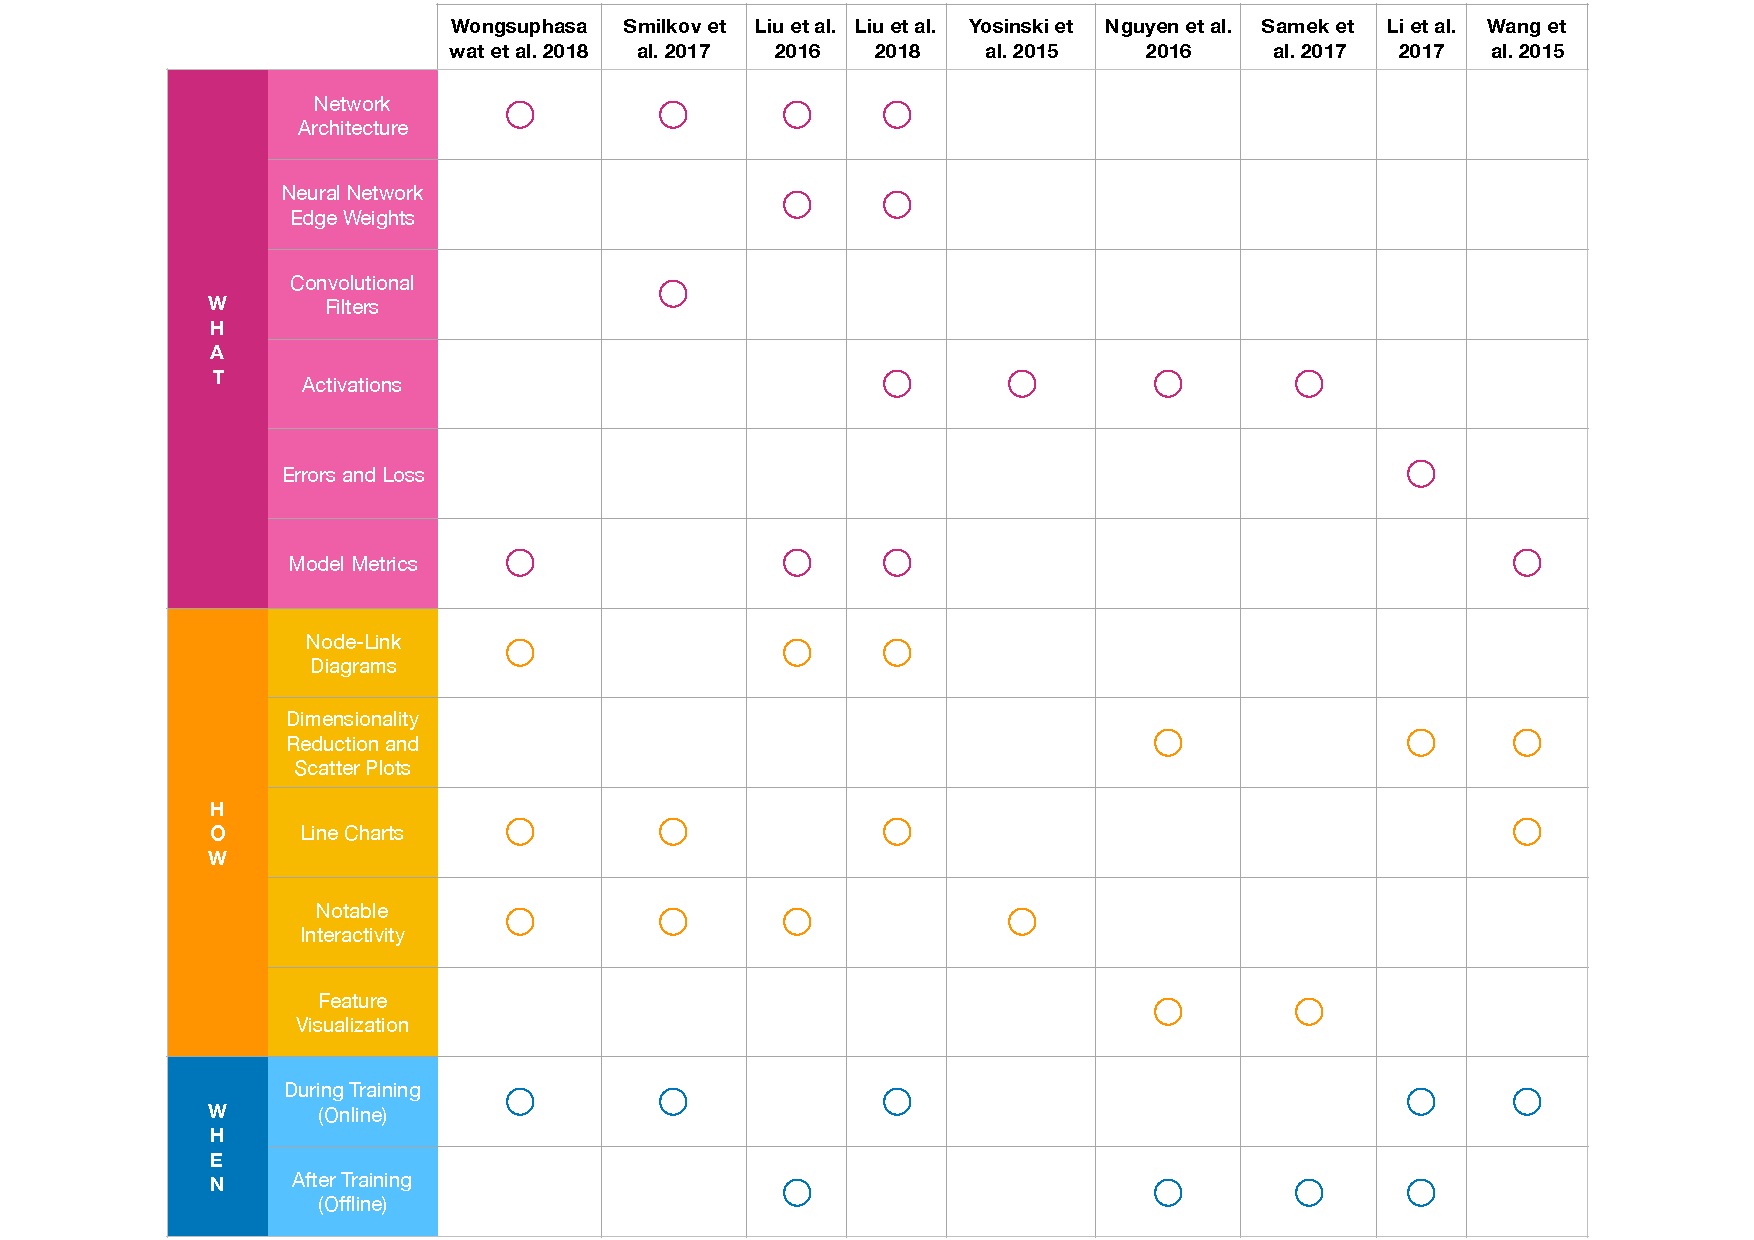
\includegraphics[width=\textwidth]{Table}
  \caption{Comparison table of the major papers discussed in this work}
  \label{fig:comparison}
\end{figure}

\end{document}